\chapter{Resultados}\label{cap:resultados}
\graphicspath{{chapter-07/img-cap07/}}

O programa FLUENT 2021R2 \cite{fluent2021ansys} foi utilizado para implementação de malha, resolução do sistema de equações algébricas e pós-processamento das simulações de dinâmica dos fluidos computacional. As simulações CFD analisam as configurações com e sem \textit{Base Bleed} (ativo e inerte, respectivamente), assim como três parâmetros do projetil ativo: o diâmetro de saída; a vazão mássica e a temperatura. Também é verificada a diferença entre os resultados das análises feitas a partir de dois modelos RANS de turbulência (Spalart-Allmaras e SST \(\kappa-\omega\)) para a munição ativa numa configuração específica.

Os valores encontrados para as curvas de arrasto em função do número de Mach foram acoplados a um código desenvolvido em MATLAB® para fazer a predição de trajetória. A validação do programa foi desenvolvida pela comparação dos resultados de uma tabela de tiro para uma munição \qty{155}{\millimetre} e do PRODAS®. Deste ponto em diante foram elaboradas trajetórias com dois ângulos de elevação (\qtylist{711;800}{\milliradian}) para averiguar a extensão de alcance para um projetil ativo sobre o caso inerte.

\section{Projetil inerte (sem \textit{Base Bleed})}\label{sec:resultados-sem-basebleed}

Os valores encontrados para o coeficiente de arrasto aerodinâmico em um projetil de artilharia sem uso de \textit{Base Bleed} foram desenvolvidos a partir do modelo SST \(\kappa-\omega\), como visto na \autoref{fig:cd-sembasebleed-comparacao}. As curvas de arrasto foram desenvolvidas com base nas malhas citadas na \autoref{tab:tabela-malhas-inicial} e foram comparadas com os resultados obtidos em simulação computacional desenvolvida por \citeauthor{Mahmoud2009}. 

\begin{figure}[!htpb]
	\centering
	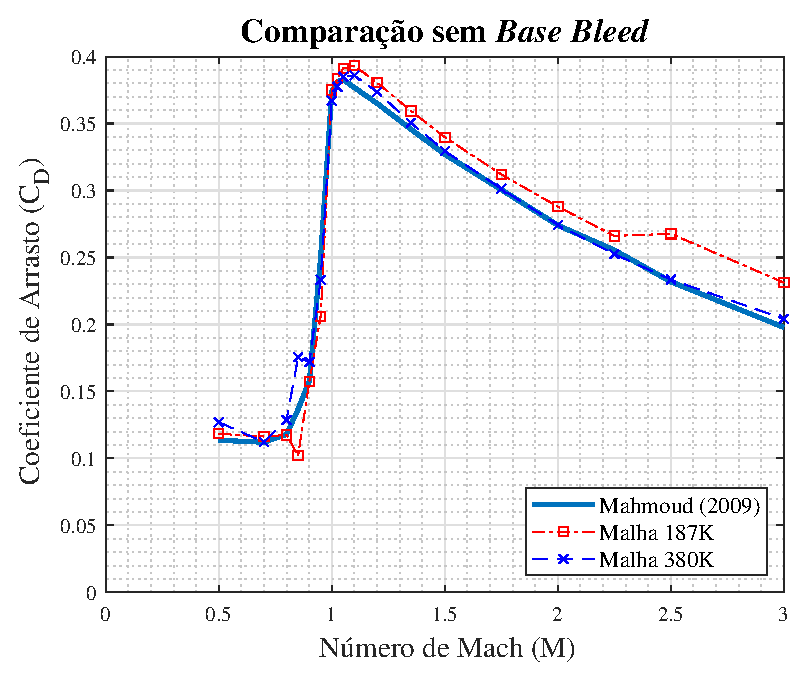
\includegraphics[width=0.5\textwidth]{cd-sembasebleed-comparacao.eps}
	\caption{Coeficiente de Arrasto \(C_{D}\) em função do número de Mach (sem BB)}
	\label{fig:cd-sembasebleed-comparacao}
\end{figure}

Através do que é demonstrado na \autoref{fig:cd-sembasebleed-comparacao}, percebe-se que a curva referente a malha com \num{380000} elementos (380K) se aproximou consideravelmente da referência. Por esta razão, a implementação do domínio computacional serviu para validação geral das próximas análises com a tecnologia \textit{Base Bleed} como condição de contorno.

\begin{figure}[!htpb]
	\centering
	\begin{subfigure}[b]{0.47\textwidth}
        \centering
        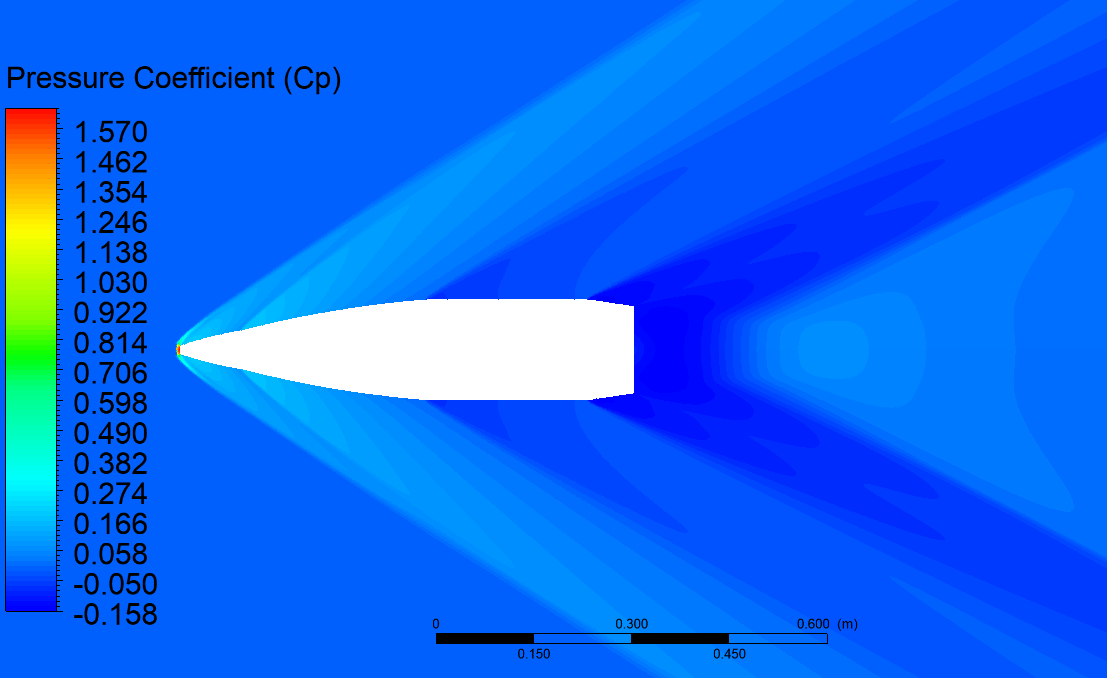
\includegraphics[height=5cm,width=\textwidth]{contorno-pressao.png}
        \caption{Contornos de pressão}
        \label{fig:contorno-pressao-sembasebleed}
    \end{subfigure}
    \hfill
	\begin{subfigure}[b]{0.47\textwidth}
        \centering
        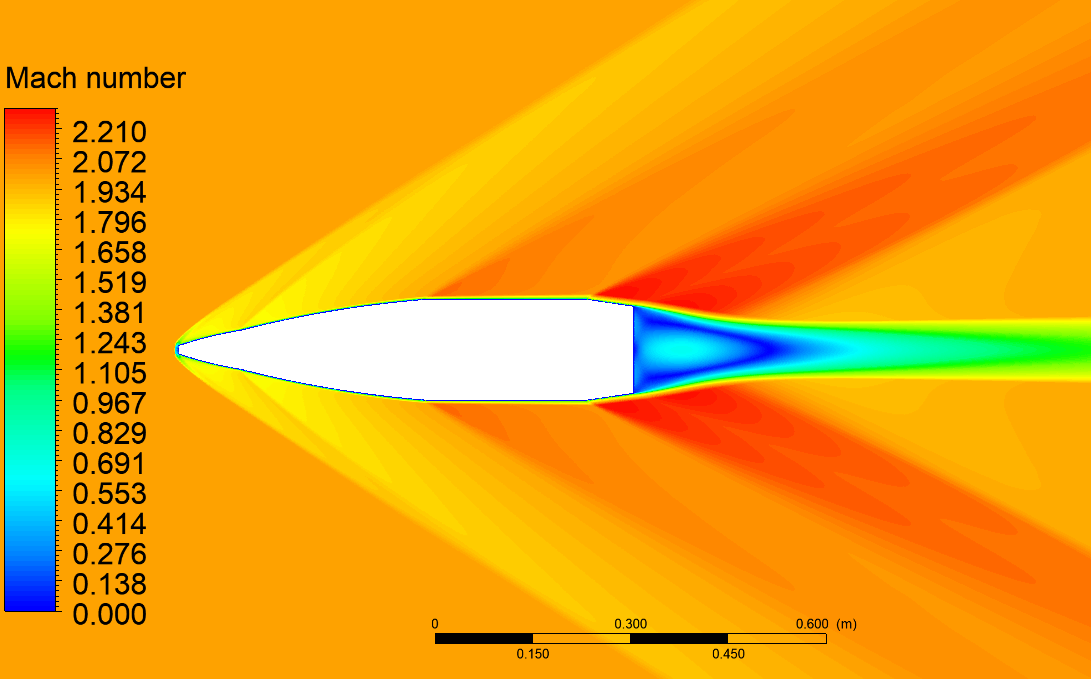
\includegraphics[height=5cm,width=\textwidth]{contorno-velocidade.png}
        \caption{Contornos de velocidade}
        \label{fig:contorno-velocidade-sembasebleed}
    \end{subfigure}
	\caption{Projetil sob regime de velocidade igual a Mach \num{2}}
	\label{fig:contornos-pressao-velocidade-sembasebleed}
\end{figure}

Antes de iniciar as validações das simulações que incluem o efeito \textit{Base Bleed}, observou-se a onda de choque da \autoref{fig:contornos-pressao-velocidade-sembasebleed}, que é causada pela velocidade supersônica (M = \num{2,0}). Além disso, há a separação da fluido com a parede na região a jusante do projetil, onde existe uma região de baixa pressão na base da munição cuja consequência é criar uma região de recirculação com baixas velocidades. A \autoref{fig:campos-pressao-velocidade-base-sembasebleed} apresenta o detalhamento na região de maior interesse, pois a tecnologia \textit{Base Bleed} procura reduzir o arrasto total através da diminuição do arrasto causado pela pressão atmosférica na base do projetil. Na \autoref{fig:corrente-velocidade-base-sembasebleed} se atesta as linhas de corrente para verificar a formação da bolha de recirculação, enquanto que o campo de pressão é relatado na \autoref{fig:contorno-pressao-base-sembasebleed} para analisar a influência do gradiente existente sob a região.

\begin{figure}[!htpb]
    \centering
    \begin{subfigure}[b]{0.47\textwidth}
        \centering
        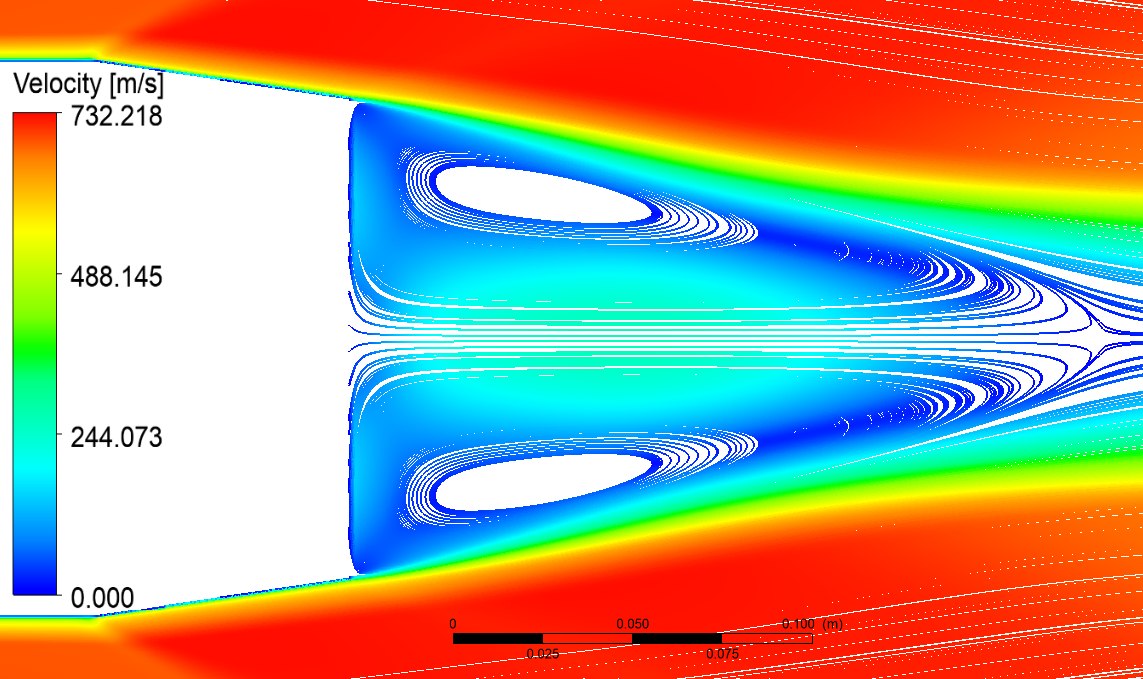
\includegraphics[height=5cm,width=\textwidth]{corrente-velocidade-off.png}
        \caption{Linhas de corrente de velocidade para a base do projetil}
        \label{fig:corrente-velocidade-base-sembasebleed}    
    \end{subfigure}
    \hfill
    \begin{subfigure}[b]{0.47\textwidth}
        \centering    
        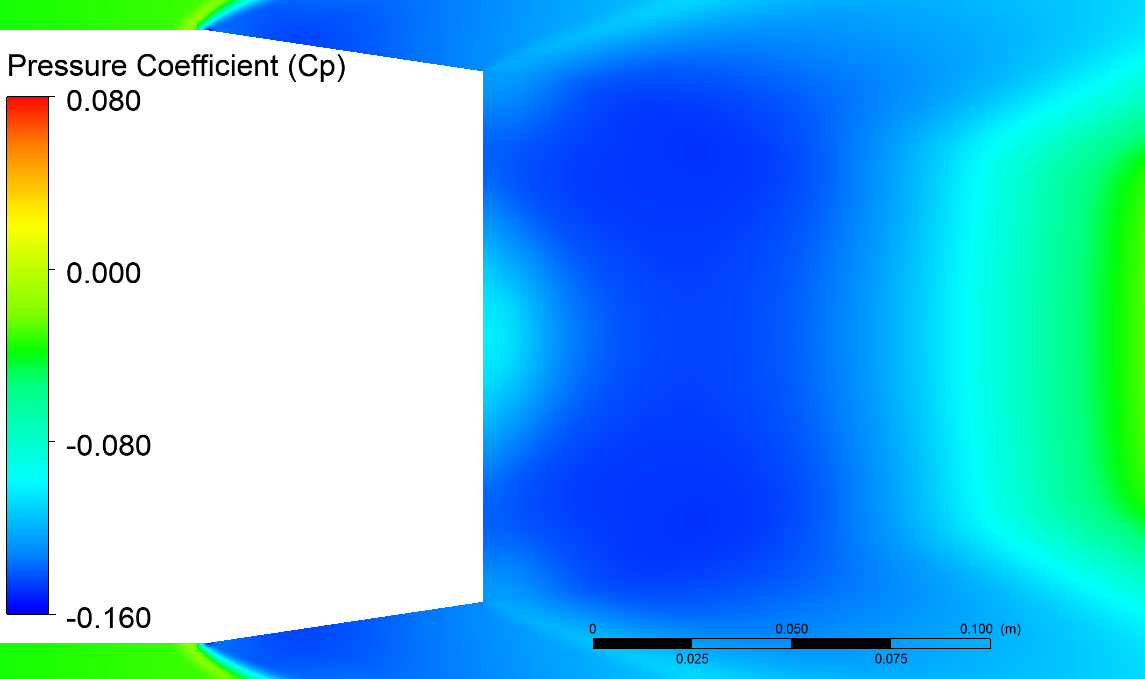
\includegraphics[height=5cm,width=\textwidth]{coeficientepressao-INERTE.png}
        \caption{Contornos de pressão para a base do projetil}
        \label{fig:contorno-pressao-base-sembasebleed}
    \end{subfigure}
    \caption{Campos de pressão e velocidade para a base do projetil sob M = \num{2,0}}
    \label{fig:campos-pressao-velocidade-base-sembasebleed}
\end{figure}

\section{Projetil ativo (com \textit{Base Bleed})}\label{sec:resultados-com-basebleed}

A Tabela \ref{tab:tabela-malhas-secundaria}, presente na Seção \ref{sec:geracao-malha}, demonstra as malhas testadas para o projetil ativo. A malha com \num{380000} elementos foi utilizada como referência, tendo em vista a convergência dos resultados com valores de trabalhos anteriores \cite{Mahmoud2009}. Com estas malhas foram feitos testes de convergência, em dois regimes de velocidade (Mach igual a \numlist{1,0;2,0}), cujos resultados são apresentados na \autoref{tab:tabela-malhas-convergencia}. Em ambos os casos o modelo SST \(\kappa-\omega\) foi usado para descrever a turbulência. A condição de contorno "Saída do \textit{Base Bleed}"{} considerou a saída dos gases com a seguinte configuração: \(\phi_{BB} = \qty{50,8}{\milli\metre}; \Dot{m}_{BB} = \qty{0,030}{\kilogram\per\second}; T_{BB} = \qty{2306,15}{\kelvin}\).

\begin{table}[ht]
\centering
\caption[Teste de convergência (com \textit{Base Bleed})]{Teste de convergência (com \textit{Base Bleed})}
\vspace{0.5cm}
\begin{tabular}{c|c|c|c|c}
\multicolumn{5}{c}{Segundo Teste de Convergência} \\
\hline 
Número de elementos & \(C_{D}\) (M = \num{1}) & Diferença & \(C_{D}\) (M = \num{2}) & Diferença\\ 
\hline
\num{380000} & 0,32784 & -- & 0,26330 & --\\
\num{453600} & 0,33064 & \qty{0,854}{\percent} & 0,26364 & \qty{0,129}{\percent}\\
\num{514800} & 0,32912 & \qty{0,390}{\percent} & 0,26185 & \qty{0,551}{\percent}\\
\num{566550} & 0,32656 & \qty{0,394}{\percent} & 0,26143 & \qty{0,710}{\percent}\\
\end{tabular}
\label{tab:tabela-malhas-convergencia}
\fonte{Autor.}
\end{table}

Para o projetil em velocidade sônica (M = \num{1,0}), a maior diferença percentual ficou na ordem de \qty{0,85}{\percent}, enquanto que para M = \num{2,0} o maior desvio foi de aproximadamente \qty{0,7}{\percent}, o que denota quase nenhuma diferença nos resultados mesmo aumentando significativamente o número de elementos. Desta forma, o custo computacional para resolver a malha com \num{380000} elementos é suficiente para predizer o coeficiente de arrasto.

\subsection{Influência no diâmetro de saída do \textit{Base Bleed}} \label{subsec:resultados-com-basebleed-diametros}

\begin{figure}[!htpb]
	\centering
    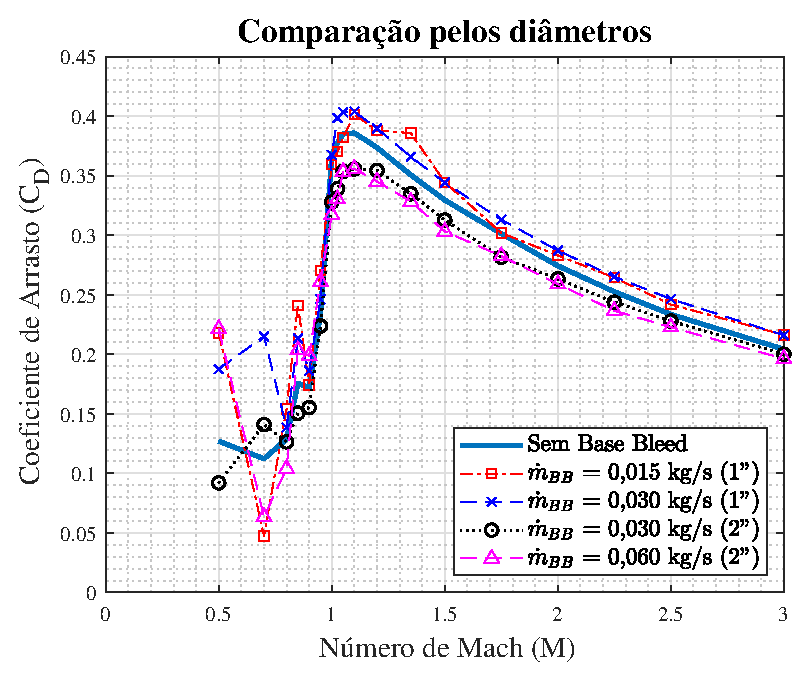
\includegraphics[width=0.5\textwidth]{cd-combasebleed-diametro-1e2pol.eps}
	\caption{Influência do diâmetro do \textit{Base Bleed}}
	\label{fig:comparacao-bb-diametro-1e2pol}
\end{figure}

O primeiro parâmetro estudado foi o aumento do diâmetro da saída do bocal (ver \autoref{tab:tabela-vazoes-por-diametro}), de \qtyrange{25,4}{50,8}{\millimetre} (de \qtyrange{1}{2}{\polegada}). A temperatura na condição de contorno "Saída do \textit{Base Bleed}"{} foi fixada em \(T_{BB} = \qty{2306,15}{\kelvin}\), conforme apresentado em \cite{Gil2020}. Desta forma, a Figura \ref{fig:comparacao-bb-diametro-1e2pol} demonstra uma redução do coeficiente de arrasto somente para o diâmetro de \qty{2}{\polegada}. O diâmetro de injeção de gases igual \qty{1}{\polegada} causou um acréscimo na força de arrasto, nas duas condições de vazão mássicas impostas, quando comparado ao sistema BB desativado. Há de se notar uma oscilação presente nas curvas de arrasto no regime subsônico com o \textit{Base Bleed} funcionando, especialmente na faixa M < \num{0,8}.

Para entender o acréscimo de arrasto nos projetis com diâmetro de saída do \textit{Base Bleed} iguais a \qty{1}{\polegada} \(\left(\phi_{BB} = \qty{25,4}{\millimetre}\right)\), a \autoref{fig:influencia-diametro-vazao-1pol} apresenta os campos de pressão e velocidade sob regime M = \num{2,0}. As Figuras \ref{fig:contorno-pressao-bb-1pol-vazao0015} e \ref{fig:contorno-pressao-bb-1pol-vazao0030} demonstram o campo de pressão no entorno do projetil, cujos valores mínimos encontram-se na base do projetil. As Figuras \ref{fig:contorno-pressao-base-bb-1pol-vazao0015} e \ref{fig:contorno-pressao-base-bb-1pol-vazao0030} apresentam o campo de pressão a jusante do projetil, onde se relata valores mais baixos para a pressão na \autoref{fig:contorno-pressao-base-bb-1pol-vazao0030}.  

As consequências desses campos de pressão podem ser observados nos campos de velocidades, representados ao longo de toda a munição (ver Figuras \ref{fig:contorno-velocidade-bb-1pol-vazao0015} e \ref{fig:contorno-velocidade-bb-1pol-vazao0030}) e especificamente para a base deste projetil (ver Figuras \ref{fig:corrente-velocidade-bb-1pol-vazao0015} e \ref{fig:corrente-velocidade-bb-1pol-vazao0030}). As linhas de corrente permitem concluir que formaram-se zonas de recirculação, como as previstas por \cite{Sahu1985}, mas a Figura~\ref{fig:corrente-velocidade-bb-1pol-vazao0030} apresenta uma concentração de momento linear localizada na saída dos gases. Deste fato conclui-se que há necessidade de controlar a injeção de gases de acordo com o diâmetro de saída, ou seja, um valor ideal para a vazão mássica para reduzir o arrasto, assim como foi estabelecido em referências anteriores \cite{Andersson1976,Gunners1988}. 

%%% EFEITO DIAMETRO - TEMPERATURA DE 2306K PARA O BASE BLEED 1 POLEGADA

\begin{figure}[!ht]
	\centering
	\begin{subfigure}[b]{0.47\textwidth} % CAMPO DE PRESSAO - VAZAO 15 G/S (1 POL)
        \centering
        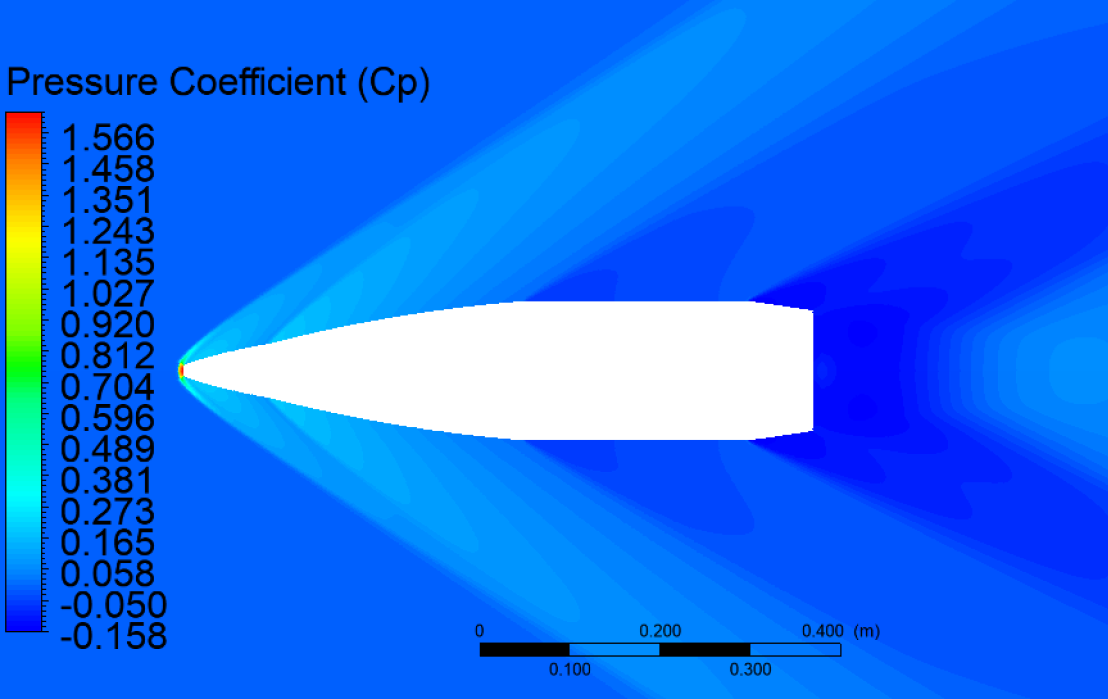
\includegraphics[height=5cm,width=\textwidth]{contorno-pressao-2306-vazao-0015-1pol.png}
        \caption{Contornos de pressão - \(\Dot{m}_{BB}\) = \qty{0,015}{\kilogram\per\second}}
        \label{fig:contorno-pressao-bb-1pol-vazao0015}
    \end{subfigure}
    \hfill
    \begin{subfigure}[b]{0.47\textwidth} % CAMPO DE PRESSAO - VAZAO 30 G/S (1 POL)
        \centering
        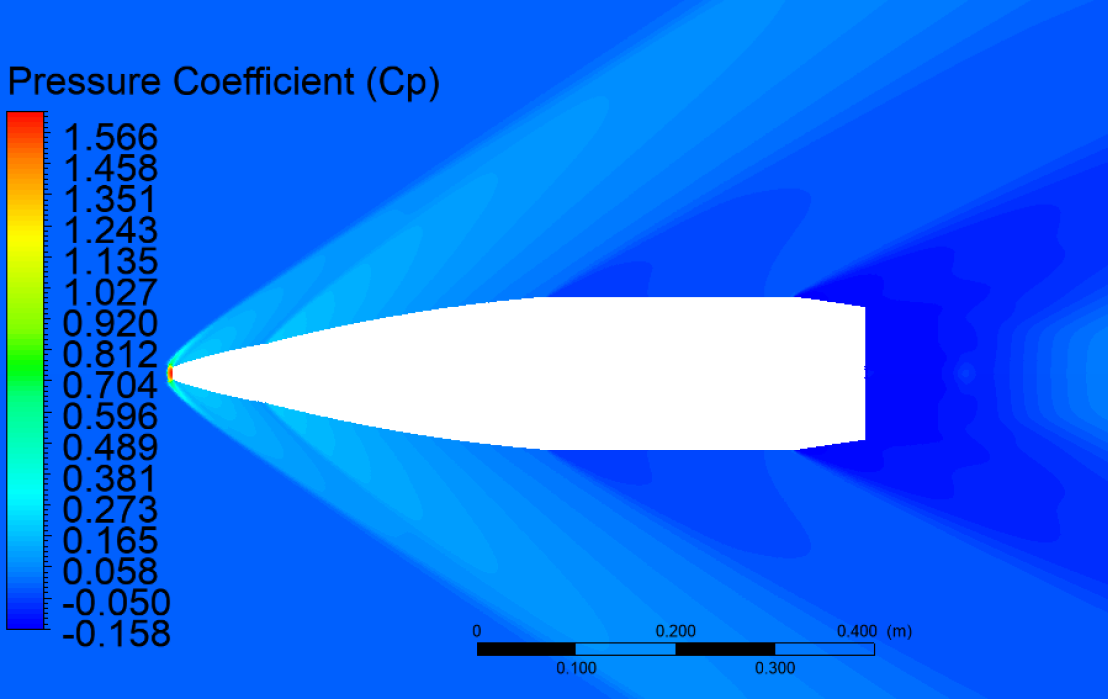
\includegraphics[height=5cm,width=\textwidth]{contorno-pressao-2306-vazao-0030-1pol.png}
        \caption{Contornos de pressão - \(\Dot{m}_{BB}\) = \qty{0,030}{\kilogram\per\second}}
        \label{fig:contorno-pressao-bb-1pol-vazao0030}
    \end{subfigure}
    \hfill
    \begin{subfigure}[b]{0.47\textwidth} % CAMPO DE PRESSAO NA BASE - VAZAO 15 G/S (1 POL)
        \centering
        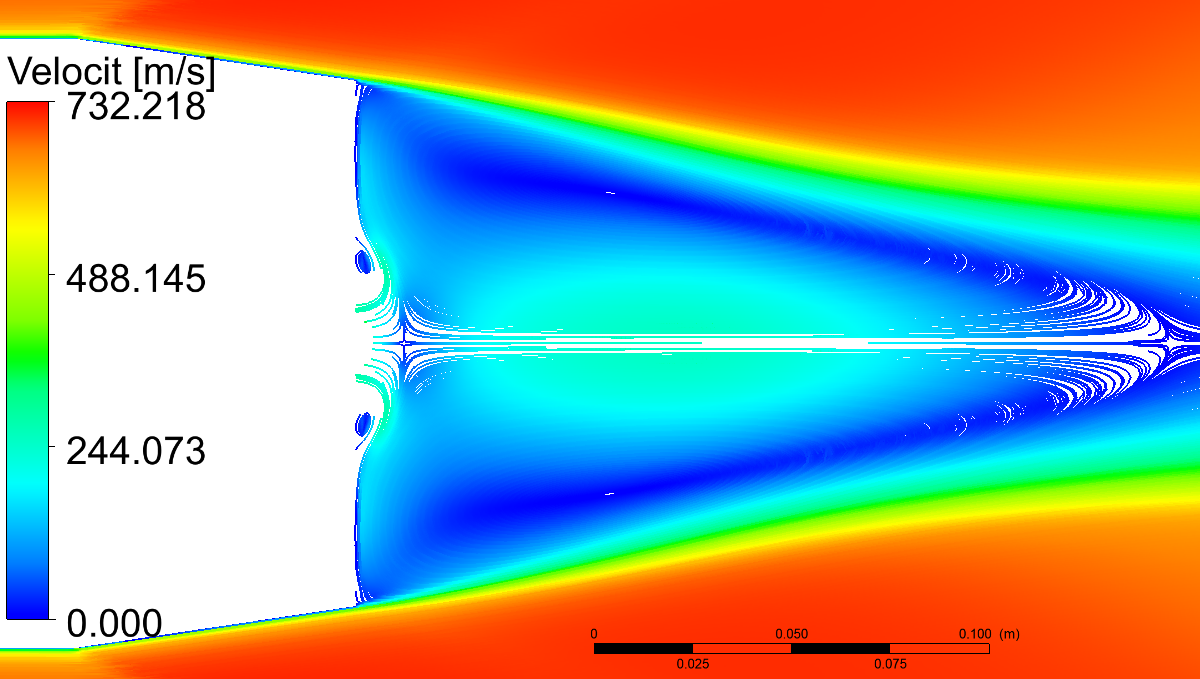
\includegraphics[height=5cm,width=\textwidth]{coeficientepressao-vazao0015-temp2306-diam1pol.png}
        \caption{Contornos de pressão - \(\Dot{m}_{BB}\) = \qty{0,015}{\kilogram\per\second}}
        \label{fig:contorno-pressao-base-bb-1pol-vazao0015}
    \end{subfigure}
    \hfill
    \begin{subfigure}[b]{0.47\textwidth} % CAMPO DE PRESSAO NA BASE - VAZAO 30 G/S (1 POL)
        \centering
        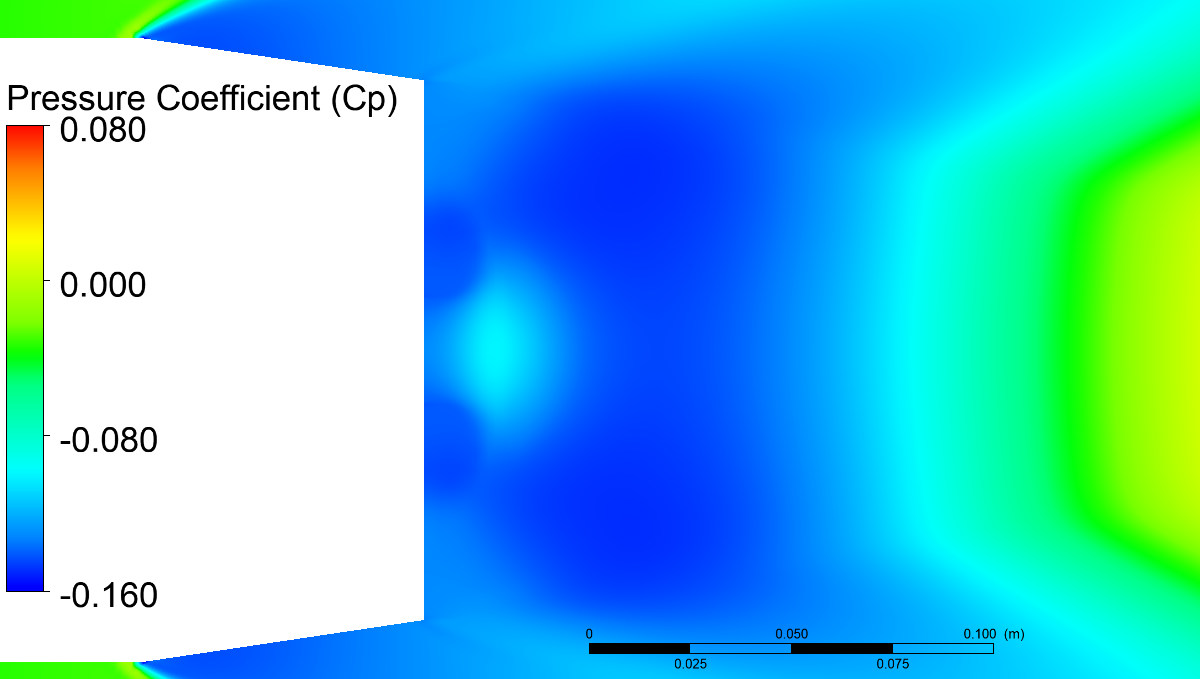
\includegraphics[height=5cm,width=\textwidth]{coeficientepressao-vazao0030-temp2306-diam1pol.png}
        \caption{Contornos de pressão - \(\Dot{m}_{BB}\) = \qty{0,030}{\kilogram\per\second}}
        \label{fig:contorno-pressao-base-bb-1pol-vazao0030}
    \end{subfigure}
    \hfill
    \begin{subfigure}[b]{0.47\textwidth} % CAMPO DE VELOCIDADE - VAZAO 15 G/S (1 POL)
        \centering
        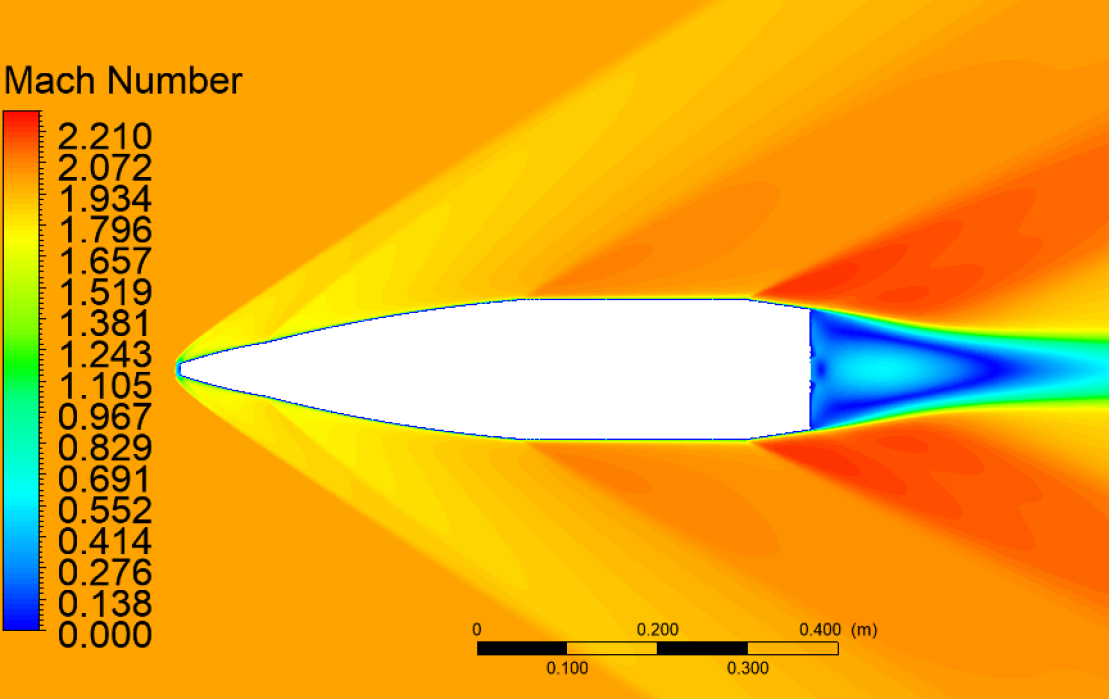
\includegraphics[height=5cm,width=\textwidth]{contorno-velocidade-2306K-vazao-0015-1pol.png}
        \caption{Cont. de velocidade - \(\Dot{m}_{BB}\) = \qty{0,015}{\kilogram\per\second}}
        \label{fig:contorno-velocidade-bb-1pol-vazao0015}
    \end{subfigure}
    \hfill
	\begin{subfigure}[b]{0.47\textwidth} % CAMPO DE VELOCIDADE - VAZAO 30 G/S (1 POL)
        \centering
        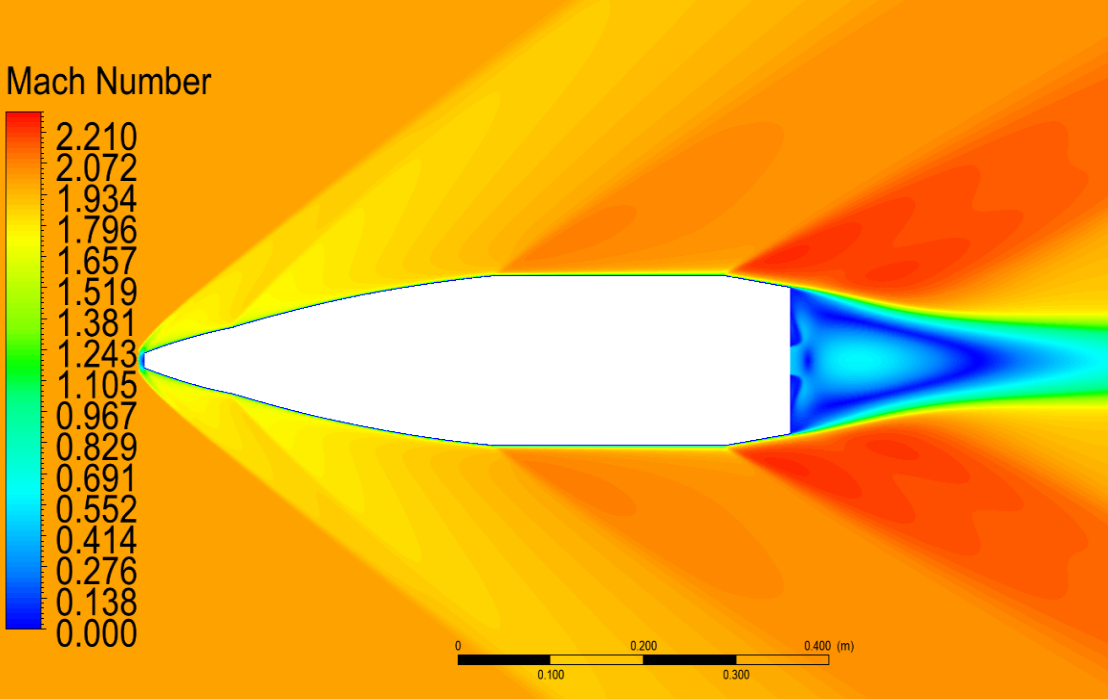
\includegraphics[height=5cm,width=\textwidth]{contorno-velocidade-2306K-vazao-0030-1pol.png}
        \caption{Cont. de velocidade - \(\Dot{m}_{BB}\) = \qty{0,030}{\kilogram\per\second}}
        \label{fig:contorno-velocidade-bb-1pol-vazao0030}
    \end{subfigure}
    \hfill
    \begin{subfigure}[b]{0.47\textwidth} % LINHAS DE CORRENTE - VAZAO 15 G/S (1 POL)
        \centering
        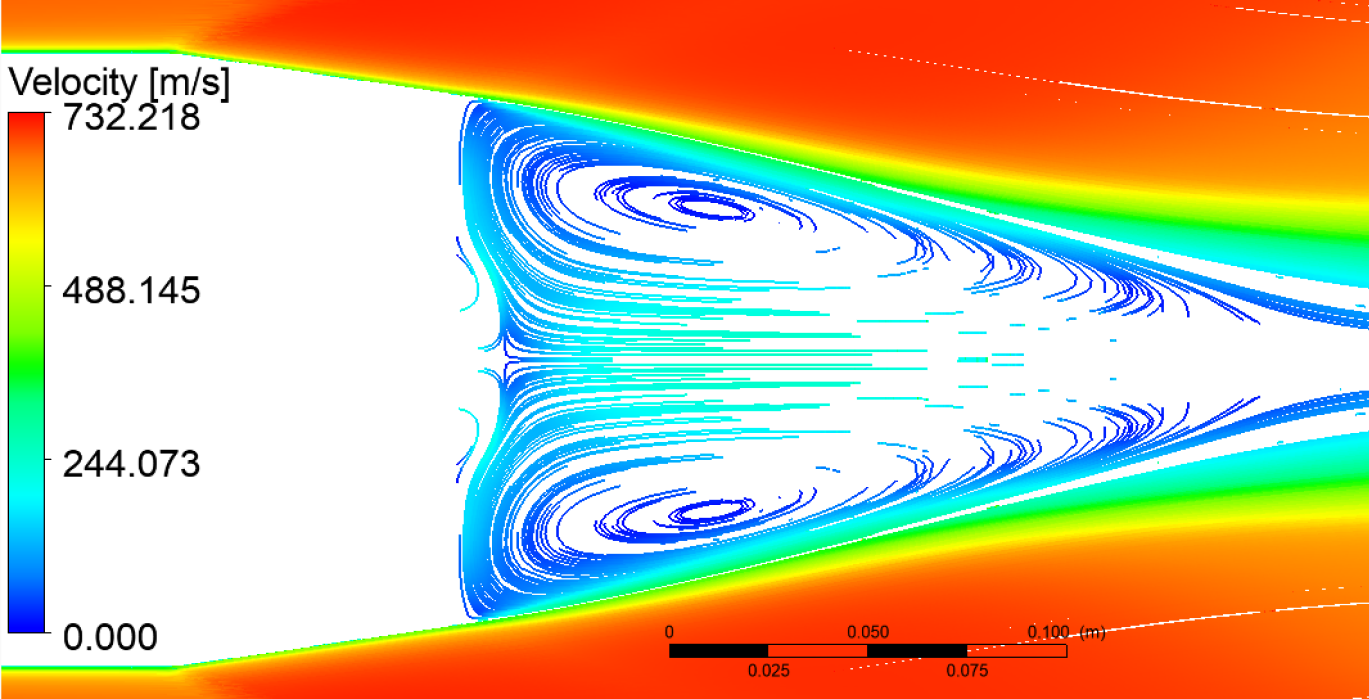
\includegraphics[height=5cm,width=\textwidth]{corrente-velocidade-2306K-vazao-0015-1pol.png}
        \caption{Linhas de corrente - \(\Dot{m}_{BB}\) = \qty{0,015}{\kilogram\per\second}}
        \label{fig:corrente-velocidade-bb-1pol-vazao0015}
    \end{subfigure}
    \hfill
    \begin{subfigure}[b]{0.47\textwidth} % LINHAS DE CORRENTE - VAZAO 30 G/S (1 POL)
        \centering
        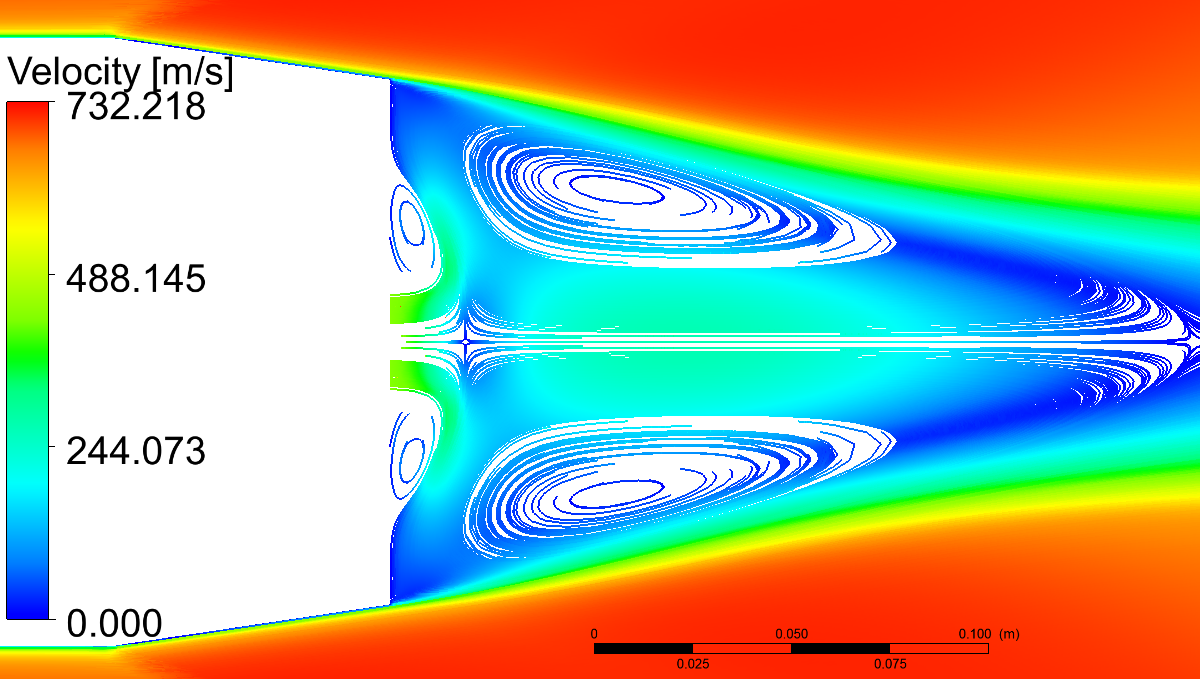
\includegraphics[height=5cm,width=\textwidth]{corrente-velocidade-2306K-vazao-0030-1pol.png}
        \caption{Linhas de corrente - \(\Dot{m}_{BB}\) = \qty{0,030}{\kilogram\per\second}}
        \label{fig:corrente-velocidade-bb-1pol-vazao0030}
    \end{subfigure}
    \caption{Campos de pressão e velocidade \(\left(\phi_{BB} = \qty{25,4}{\millimetre}; T_{BB} = \qty{2306,15}{\kelvin}\right)\)}
	\label{fig:influencia-diametro-vazao-1pol}
\end{figure}

%%% EFEITO DIAMETRO - TEMPERATURA DE 2306K PARA O BASE BLEED 2 POLEGADAS

\begin{figure}[!htpb]
	\centering
	\begin{subfigure}[b]{0.47\textwidth} % FOTO 1
        \centering
        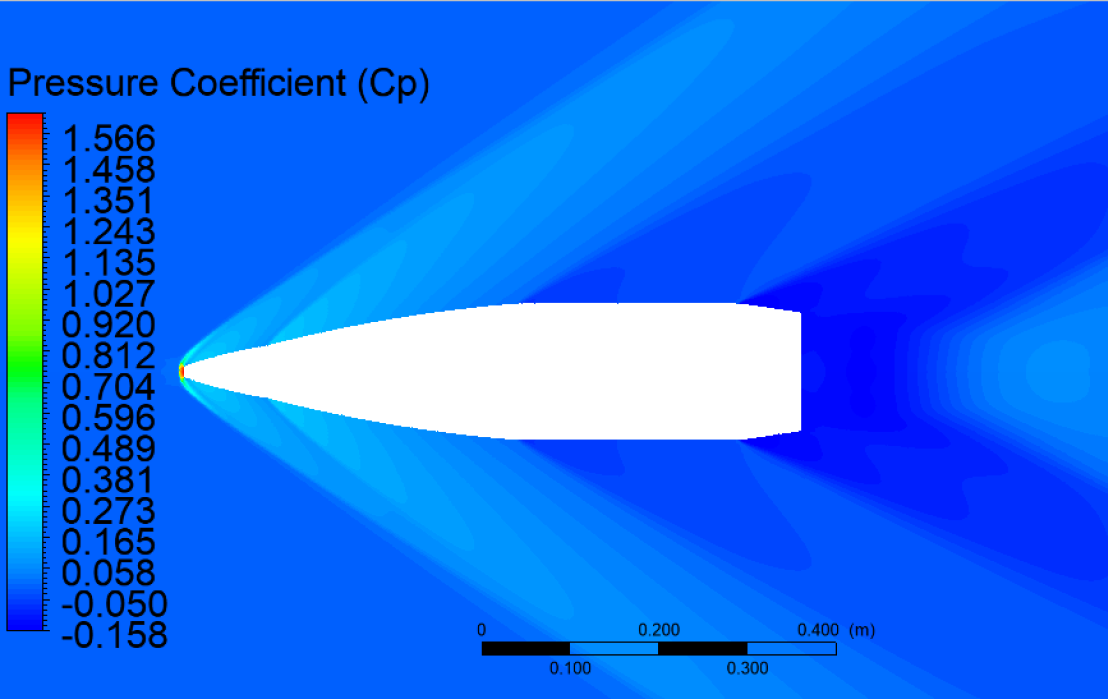
\includegraphics[height=5cm,width=\textwidth]{contorno-pressao-2306-vazao-0030-2pol.png}
        \caption{Contornos de pressão - \(\Dot{m}_{BB}\) = \qty{0,030}{\kilogram\per\second}}
        \label{fig:contorno-pressao-bb-2pol-vazao0030}
    \end{subfigure}
    \hfill
    \begin{subfigure}[b]{0.47\textwidth} % FOTO 2
        \centering
        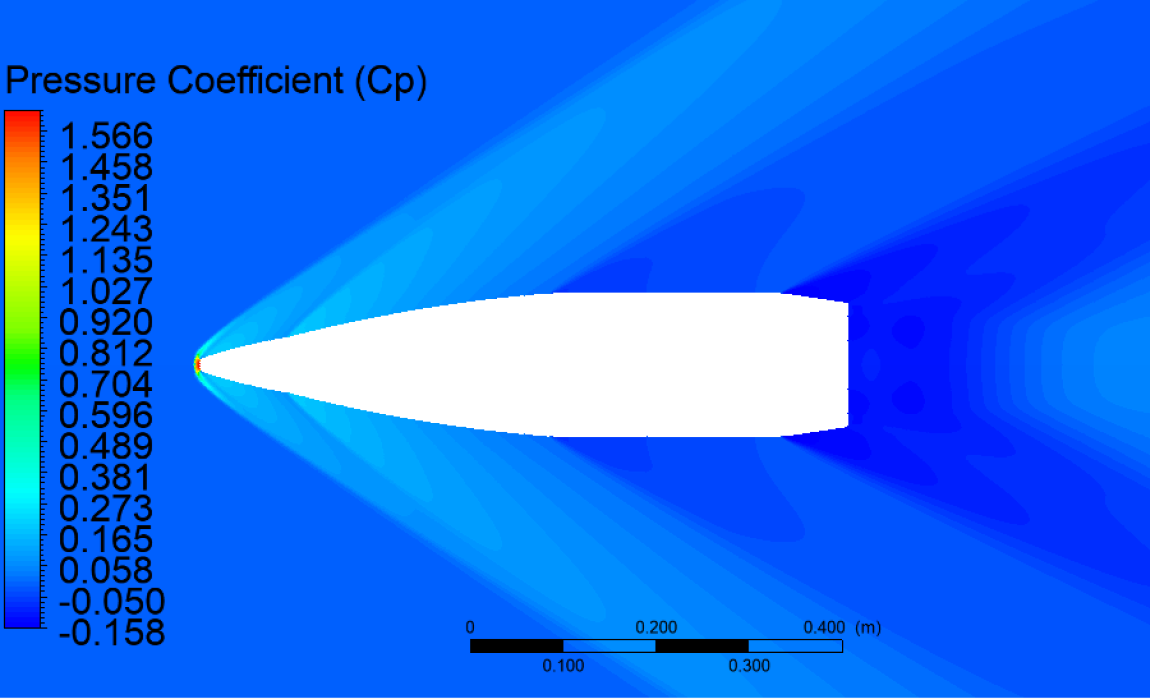
\includegraphics[height=5cm,width=\textwidth]{contorno-pressao-2306-vazao-0060-2pol.png}
        \caption{Contornos de pressão - \(\Dot{m}_{BB}\) = \qty{0,060}{\kilogram\per\second}}
        \label{fig:contorno-pressao-bb-2pol-vazao0060}
    \end{subfigure}
    \hfill
    \begin{subfigure}[b]{0.47\textwidth} % FOTO 3
        \centering
        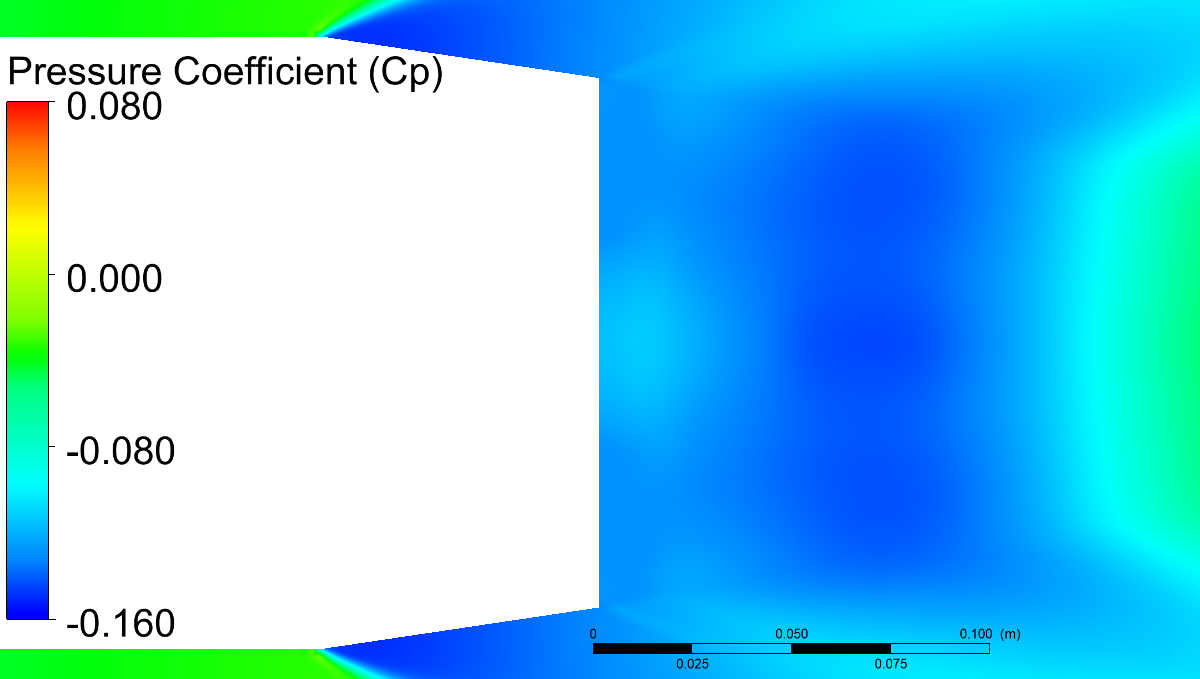
\includegraphics[height=5cm,width=\textwidth]{coeficientepressao-vazao0030-temp2306-diam2pol.png}
        \caption{Contornos de pressão - \(\Dot{m}_{BB}\) = \qty{0,030}{\kilogram\per\second}}
        \label{fig:contorno-pressao-base-bb-2pol-vazao0030}
    \end{subfigure}
    \hfill
    \begin{subfigure}[b]{0.47\textwidth} % FOTO 4
        \centering
        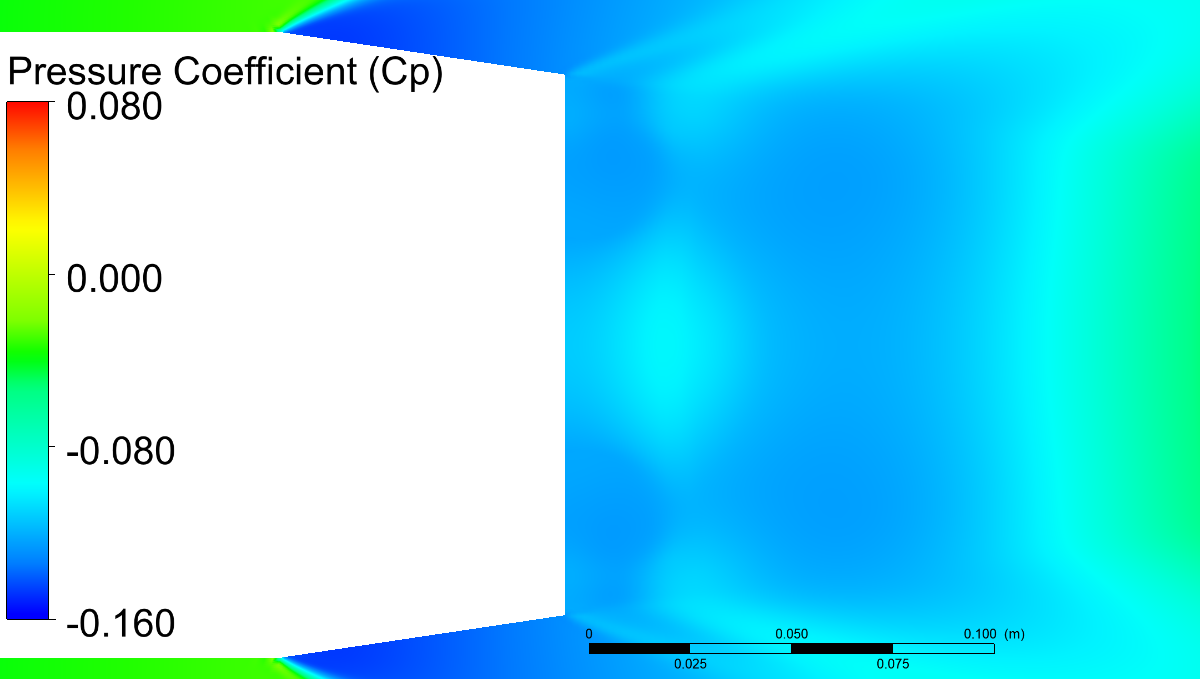
\includegraphics[height=5cm,width=\textwidth]{coeficientepressao-vazao0060-temp2306-diam2pol.png}
        \caption{Contornos de pressão - \(\Dot{m}_{BB}\) = \qty{0,060}{\kilogram\per\second}}
        \label{fig:contorno-pressao-base-bb-2pol-vazao0060}
    \end{subfigure}
    \hfill
    \begin{subfigure}[b]{0.47\textwidth} % FOTO 5
        \centering
        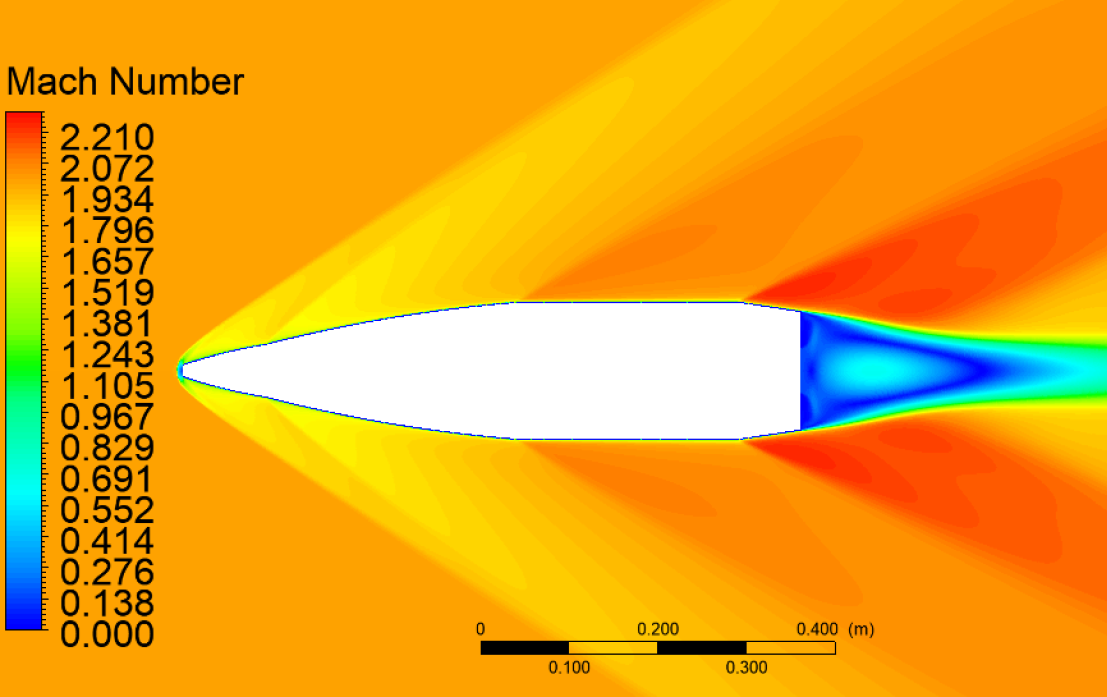
\includegraphics[height=5cm,width=\textwidth]{contorno-velocidade-2306K-vazao-0030-2pol.png}
        \caption{Cont. de velocidade - \(\Dot{m}_{BB}\) = \qty{0,030}{\kilogram\per\second}}
        \label{fig:contorno-velocidade-bb-2pol-vazao0030}
    \end{subfigure}
    \hfill
	\begin{subfigure}[b]{0.47\textwidth} % FOTO 6
        \centering
        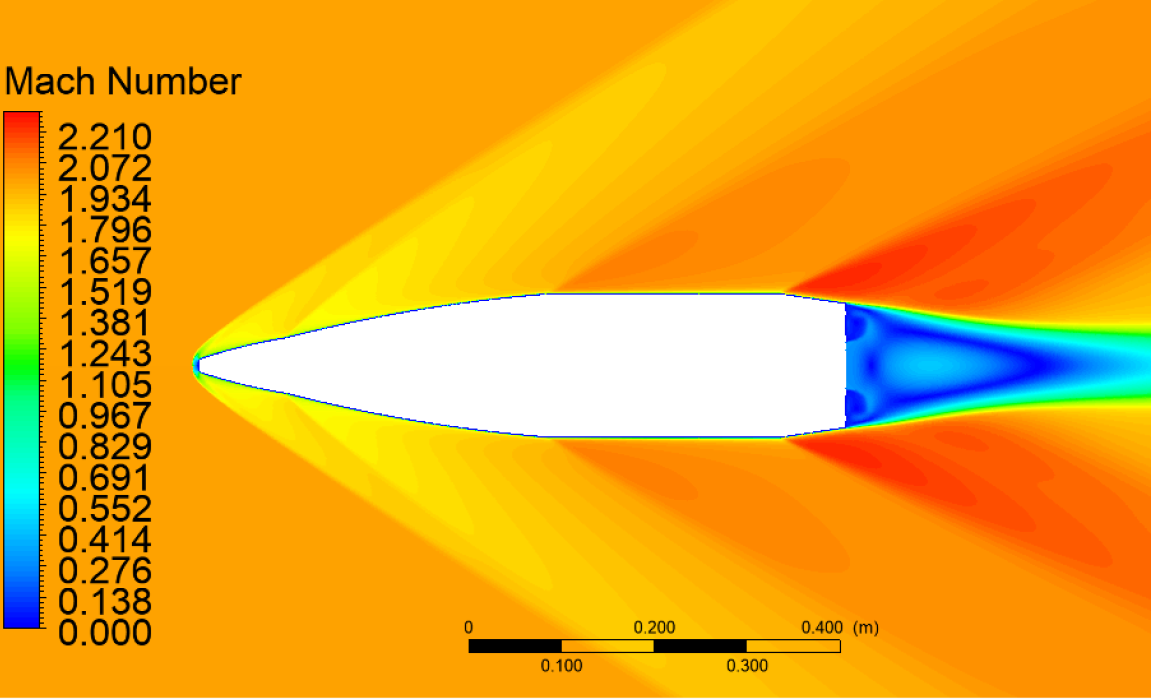
\includegraphics[height=5cm,width=\textwidth]{contorno-velocidade-2306K-vazao-0060-2pol.png}
        \caption{Cont. de velocidade - \(\Dot{m}_{BB}\) = \qty{0,060}{\kilogram\per\second}}
        \label{fig:contorno-velocidade-bb-2pol-vazao0060}
    \end{subfigure}
    \hfill
    \begin{subfigure}[b]{0.47\textwidth} % FOTO 7
        \centering
        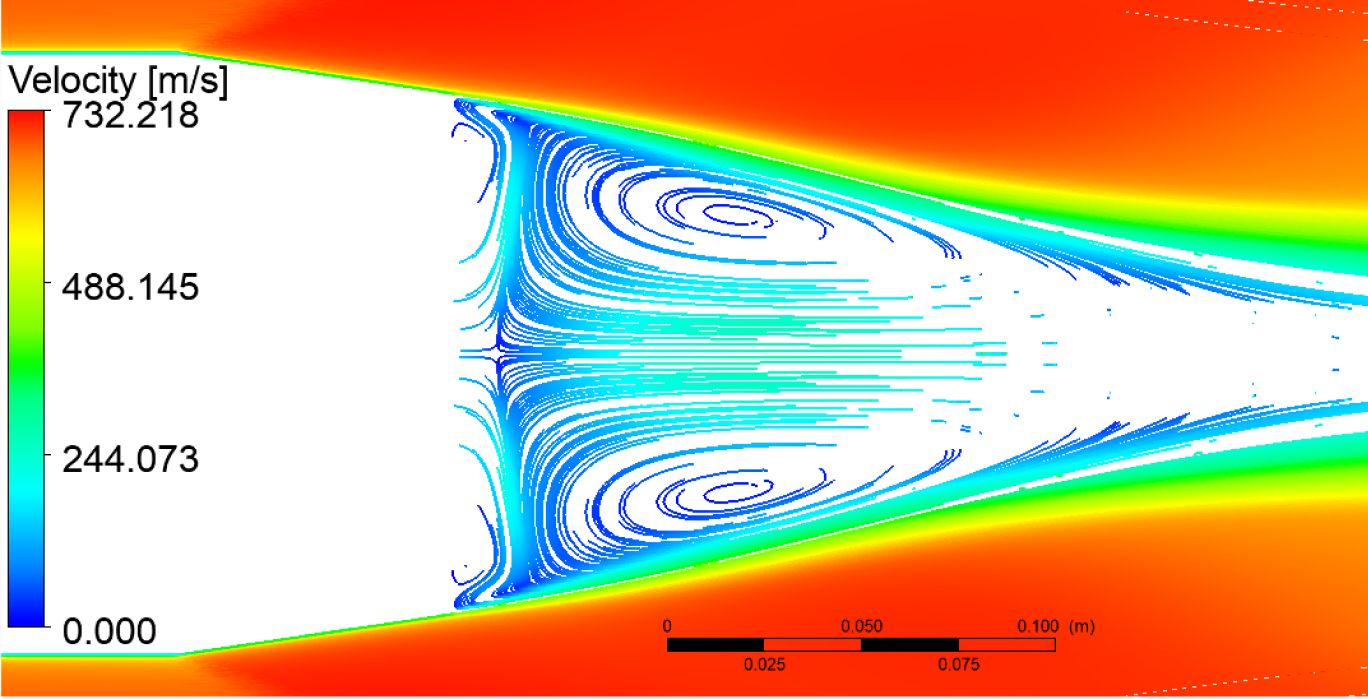
\includegraphics[height=5cm,width=\textwidth]{corrente-velocidade-2306K-vazao-0030-2pol.png}
        \caption{Linhas de corrente - \(\Dot{m}_{BB}\) = \qty{0,030}{\kilogram\per\second}}
        \label{fig:corrente-velocidade-bb-2pol-vazao0030}
    \end{subfigure}
    \hfill
    \begin{subfigure}[b]{0.47\textwidth} % FOTO 8
        \centering
        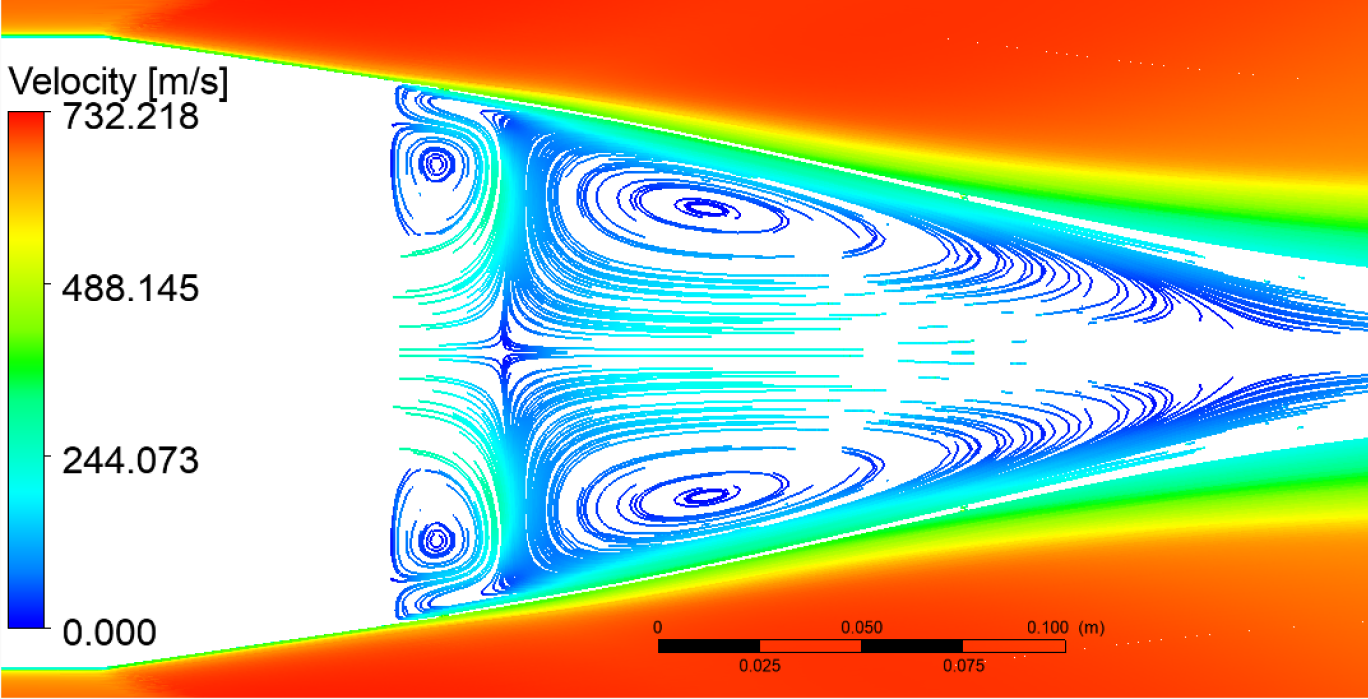
\includegraphics[height=5cm,width=\textwidth]{corrente-velocidade-2306K-vazao-0060-2pol.png}
        \caption{Linhas de corrente - \(\Dot{m}_{BB}\) = \qty{0,060}{\kilogram\per\second}}
        \label{fig:corrente-velocidade-bb-2pol-vazao0060}
    \end{subfigure}
    \caption{Campos de pressão e velocidade \(\left(\phi_{BB} = \qty{50,8}{\millimetre}; T_{BB} = \qty{2306,15}{\kelvin}\right)\)}
	\label{fig:influencia-diametro-vazao-2pol}
\end{figure}

O passo seguinte foi apresentar o escoamento no entorno do projetil assumindo que o diâmetro de saída do bocal é igual a \qty{2}{\polegada} \(\left(\phi_{BB} = \qty{50,8}{\millimetre} \right)\), conforme nota-se pela \autoref{fig:influencia-diametro-vazao-2pol}. Os campos de pressão e velocidade analisados consideraram M = \num{2,0} como condição de contorno na região "Escoamento Livre".

Os campos de pressão na base da munição apresentaram um acréscimo, sobretudo o caso da \autoref{fig:contorno-pressao-base-bb-2pol-vazao0060}. Nos campos de velocidade das Figuras \ref{fig:contorno-velocidade-bb-2pol-vazao0030} e \ref{fig:contorno-velocidade-bb-2pol-vazao0060} se observam a influência da injeção de gases na base do projetil e os detalhamentos são vistos nas linhas de correntes das Figuras \ref{fig:corrente-velocidade-bb-2pol-vazao0030} e \ref{fig:corrente-velocidade-bb-2pol-vazao0060}. Seja qual for a condição imposta para a vazão mássica \(\left(\Dot{m}_{BB} = \qtylist{0,030;0,060}{\kilogram\per\second}\right)\), os escoamentos se comportam tal como foi esquematizado pela Figura~\ref{fig3:esquemabb} \cite{Mathur&Dutton1996}. A consequência nos resultados é de maior redução nos coeficientes de arrasto durante o regime supersônico sob a seguinte configuração: \(\phi_{BB} = \qty{50,8}{\millimetre}\); \(\Dot{m}_{BB} = \qty{0,060}{\kilogram\per\second}\).

\subsection{Influência da vazão mássica no sistema \textit{Base Bleed}} \label{subsec:resultados-com-basebleed-vazao}

A \autoref{fig:comparacao-basebleed-vazao} demonstra a influência da vazão nos resultados obtidos nas simulações computacionais com o efeito \textit{Base Bleed} na base do projetil, assumindo que a temperatura de saída dos gases foi fixada em \qty{1500}{\kelvin} \cite{RosendoCILAMCE2022} e o diâmetro de saída do \textit{Base Bleed} escolhido foi de \qty{2}{\polegada} \(\left(\phi_{BB} = \qty{50,8}{\millimetre}\right)\). A escolha por esse diâmetro de saída se deve aos melhores resultados produzidos na \autoref{subsec:resultados-com-basebleed-diametros}.

Acerca do coeficiente de arrasto, nota-se na \autoref{fig:comparacao-basebleed-vazao} uma relação direta entre a redução do coeficiente de arrasto e o aumento da vazão mássica, \(\Dot{m}_{BB}\). As oscilações nos valores para o \(C_{D}\) também aparecem no regime subsônico, assim como visto na \autoref{subsec:resultados-com-basebleed-diametros}. Apesar disso, as oscilações seguem o mesmo perfil para qualquer vazão mássica imposta como condição de contorno. Sobre o regime transônico, é nele que há as maiores reduções de arrasto, no entanto, o aumento de velocidade torna o efeito \textit{Base Bleed} menos significativo, especialmente quando M > \num{2,0}.

\begin{figure}[!ht]
	\centering
	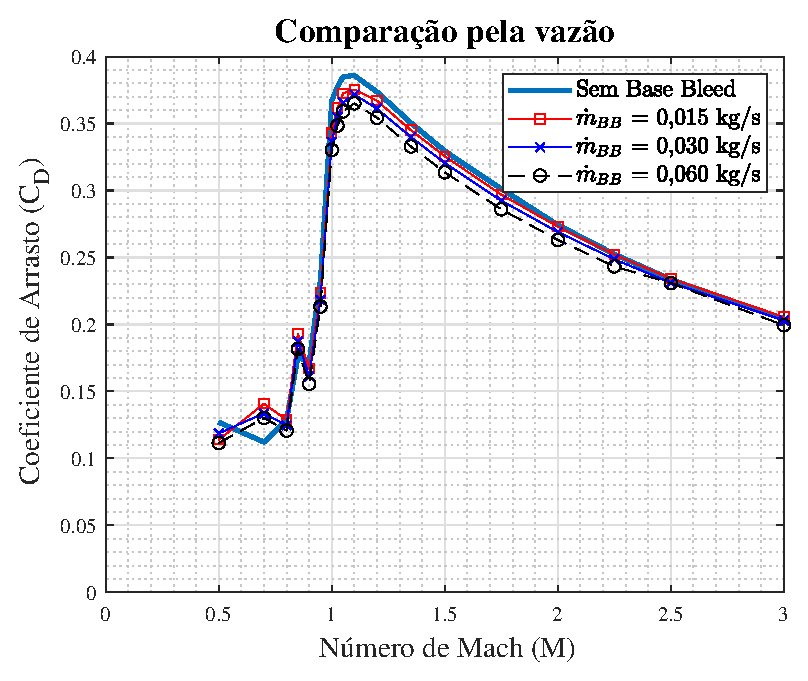
\includegraphics[width=0.5\textwidth]{cd-combasebleed-1500K-2pol.eps}
	\caption{Influência da vazão mássica do \textit{Base Bleed} - \(T_{BB}\) = \qty{1500}{\kelvin}}
	\label{fig:comparacao-basebleed-vazao}
\end{figure}

%%% EFEITO VAZAO - TEMPERATURA DE 1500K PARA O BASE BLEED 2 POLEGADAS

\begin{figure}[!htpb]
	\centering
	\begin{subfigure}[b]{0.47\textwidth} % FOTO 1
        \centering
        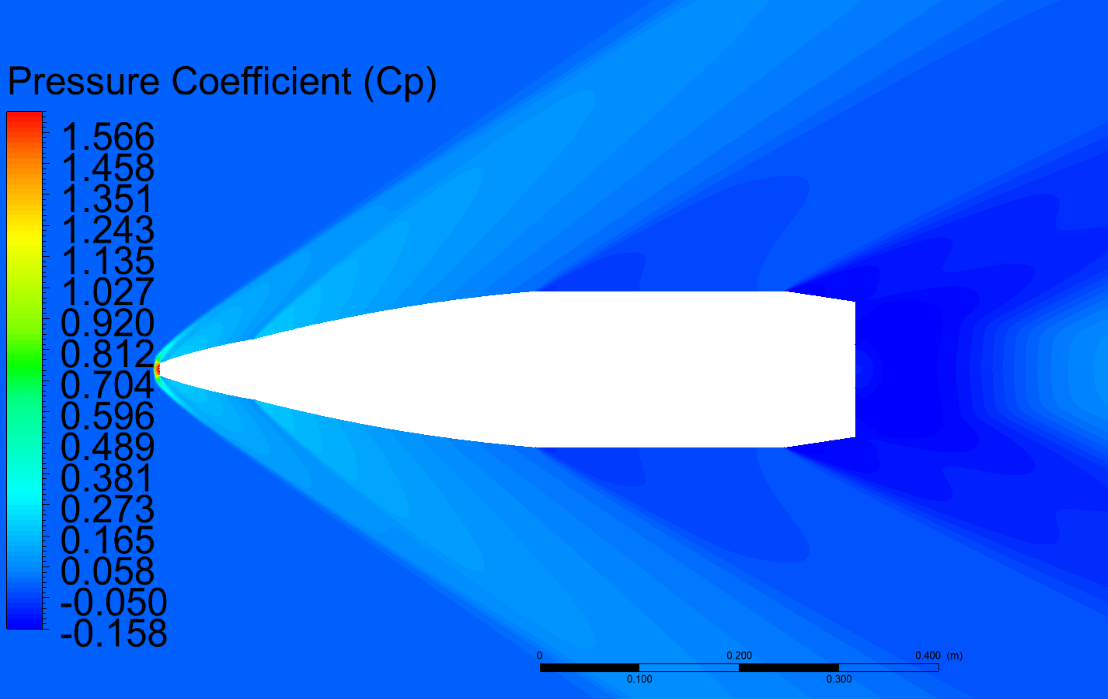
\includegraphics[height=5cm,width=\textwidth]{contorno-pressao-1500-vazao-0030-2pol.png}
        \caption{Contornos de pressão - \(\Dot{m}_{BB}\) = \qty{0,030}{\kilogram\per\second}}
        \label{fig:contorno-pressao-bb-1500K-vazao0030}
    \end{subfigure}
    \hfill
    \begin{subfigure}[b]{0.47\textwidth} % FOTO 2
        \centering
        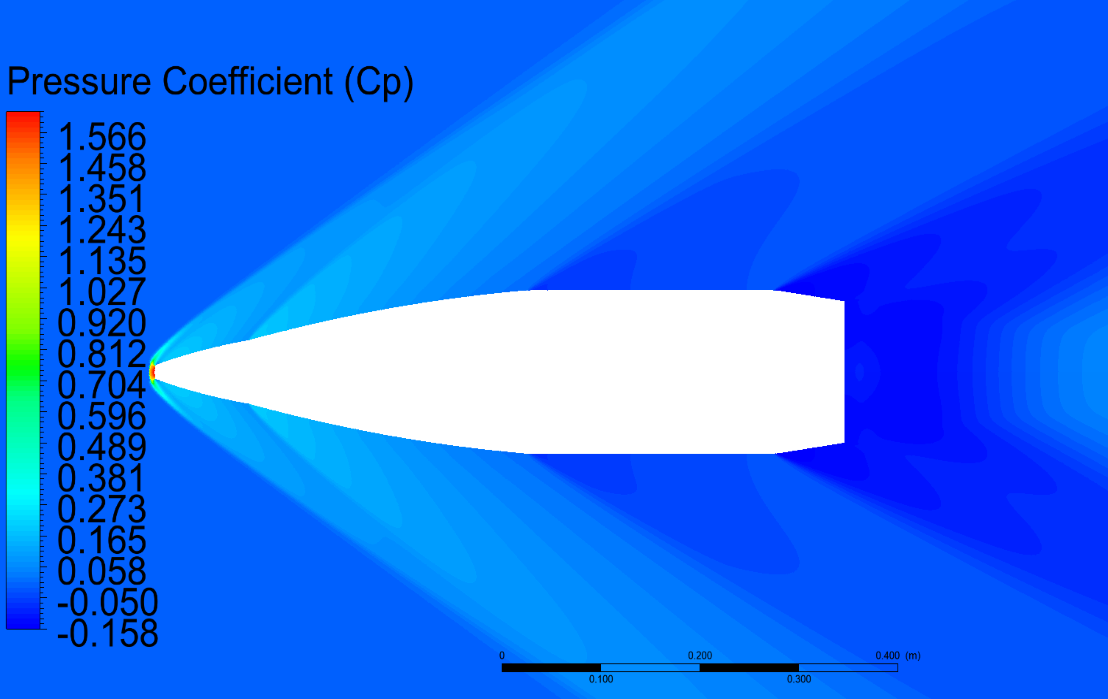
\includegraphics[height=5cm,width=\textwidth]{contorno-pressao-1500-vazao-0060-2pol.png}
        \caption{Contornos de pressão - \(\Dot{m}_{BB}\) = \qty{0,060}{\kilogram\per\second}}
        \label{fig:contorno-pressao-bb-1500K-vazao0060}
    \end{subfigure}
    \hfill
    \begin{subfigure}[b]{0.47\textwidth} % FOTO 3
        \centering
        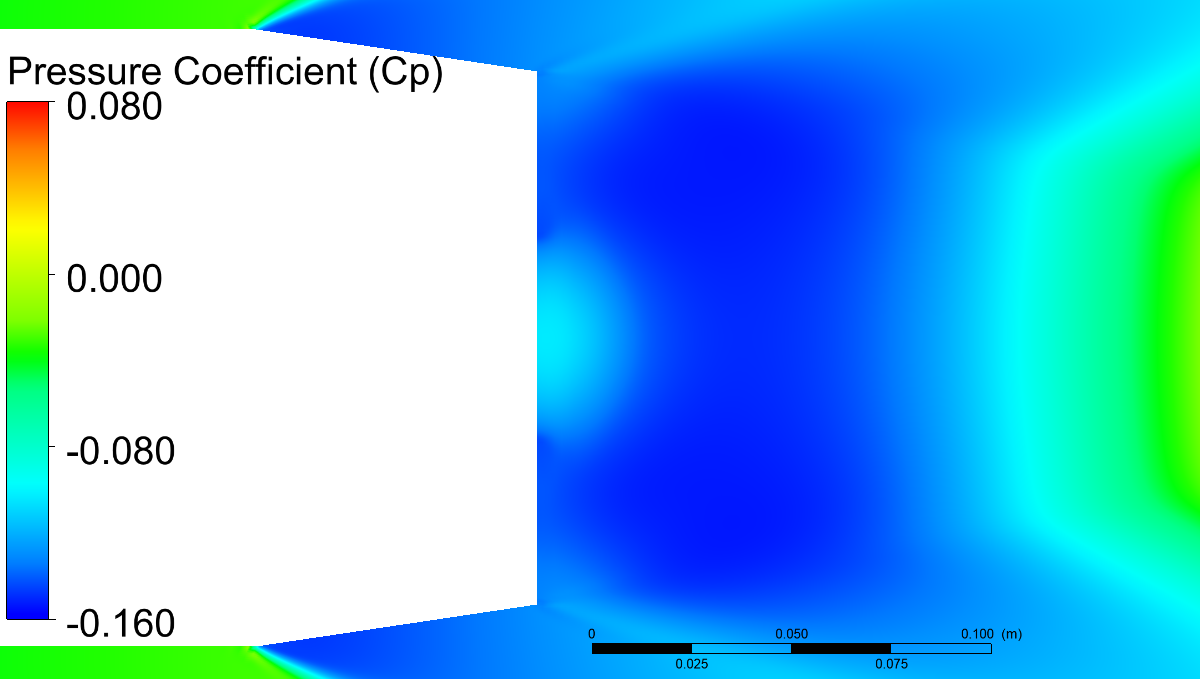
\includegraphics[height=5cm,width=\textwidth]{coeficientepressao-vazao0030-temp1500-diam2pol.png}
        \caption{Contornos de pressão - \(\Dot{m}_{BB}\) = \qty{0,030}{\kilogram\per\second}}
        \label{fig:contorno-pressao-base-bb-1500K-vazao0030}
    \end{subfigure}
    \hfill
    \begin{subfigure}[b]{0.47\textwidth} % FOTO 4
        \centering
        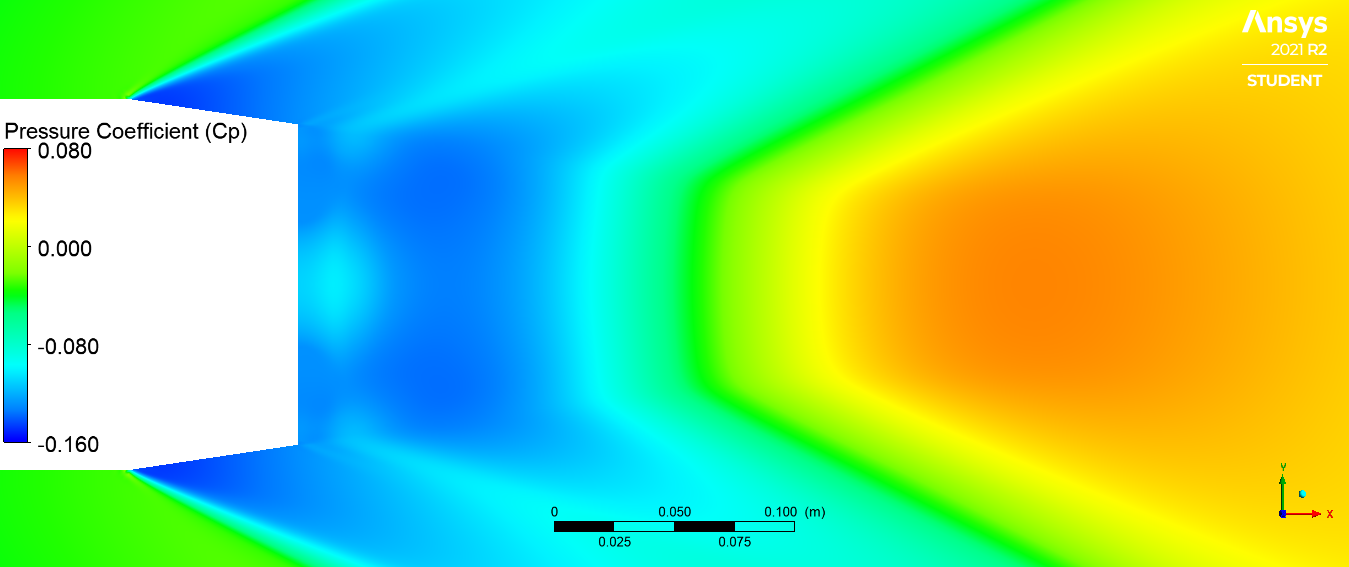
\includegraphics[height=5cm,width=\textwidth]{coeficientepressao-vazao0060-temp1500-diam2pol.png}
        \caption{Contornos de pressão - \(\Dot{m}_{BB}\) = \qty{0,060}{\kilogram\per\second}}
        \label{fig:contorno-pressao-base-bb-1500K-vazao0060}
    \end{subfigure}
    \hfill
    \begin{subfigure}[b]{0.47\textwidth} % FOTO 5
        \centering
        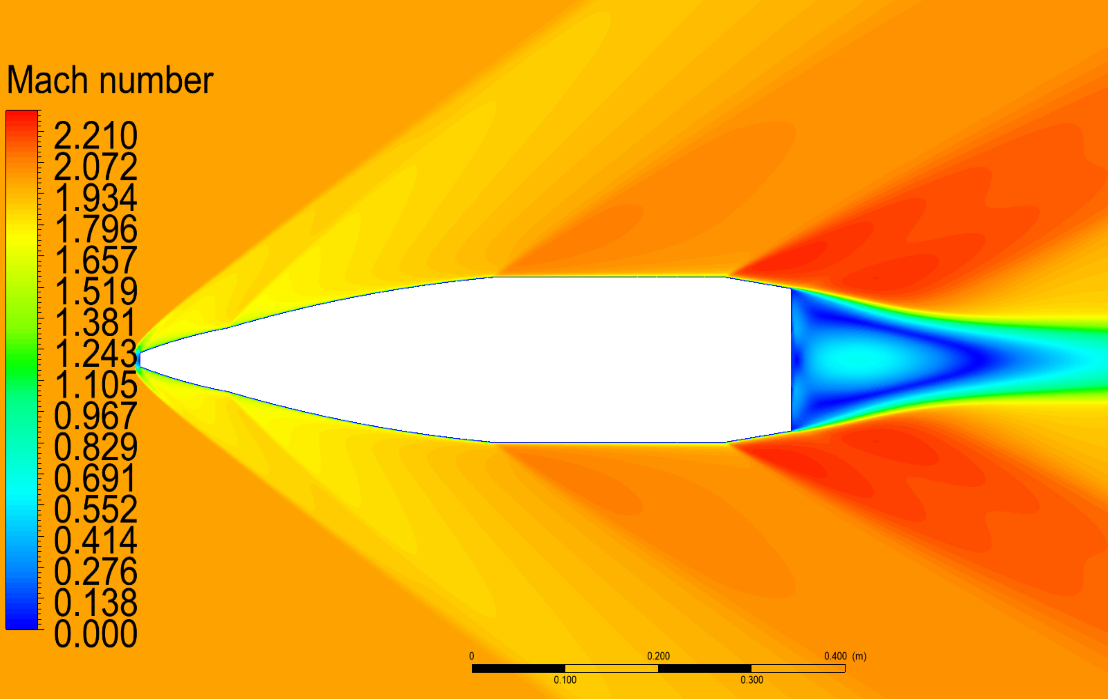
\includegraphics[height=5cm,width=\textwidth]{contorno-velocidade-1500K-vazao-0030-2pol.png}
        \caption{Cont. de velocidade - \(\Dot{m}_{BB}\) = \qty{0,030}{\kilogram\per\second}}
        \label{fig:contorno-velocidade-bb-1500K-vazao0030}
    \end{subfigure}
    \hfill
	\begin{subfigure}[b]{0.47\textwidth} % FOTO 6
        \centering
        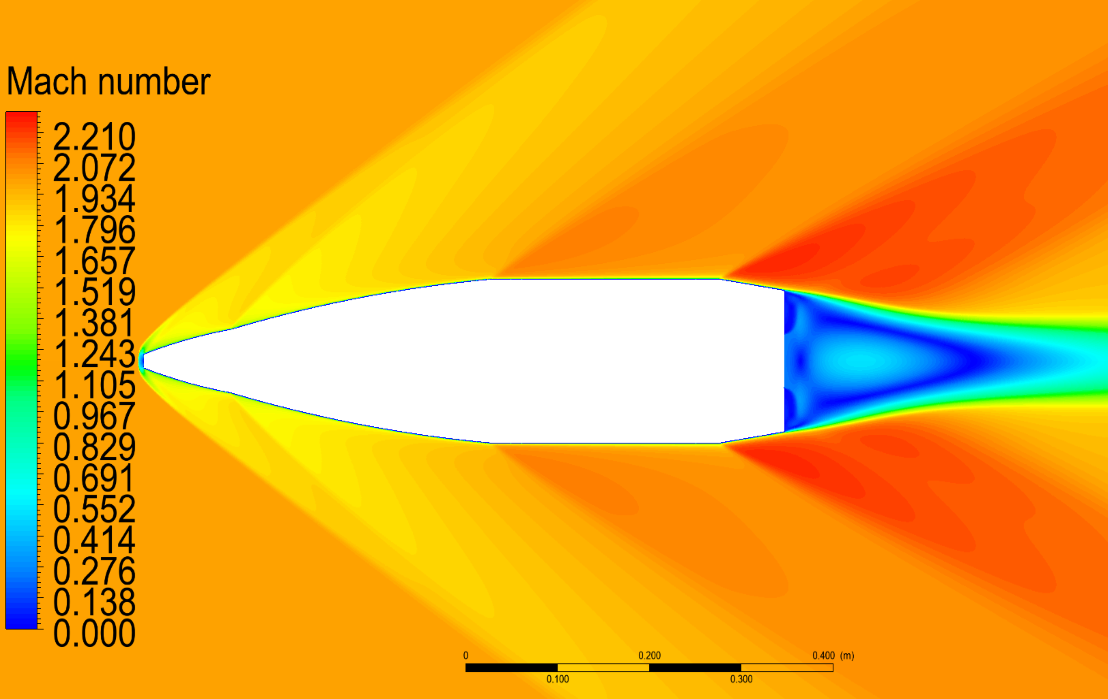
\includegraphics[height=5cm,width=\textwidth]{contorno-velocidade-1500K-vazao-0060-2pol.png}
        \caption{Cont. de velocidade - \(\Dot{m}_{BB}\) = \qty{0,060}{\kilogram\per\second}}
        \label{fig:contorno-velocidade-bb-1500K-vazao0060}
    \end{subfigure}
    \hfill
    \begin{subfigure}[b]{0.47\textwidth} % FOTO 7
        \centering
        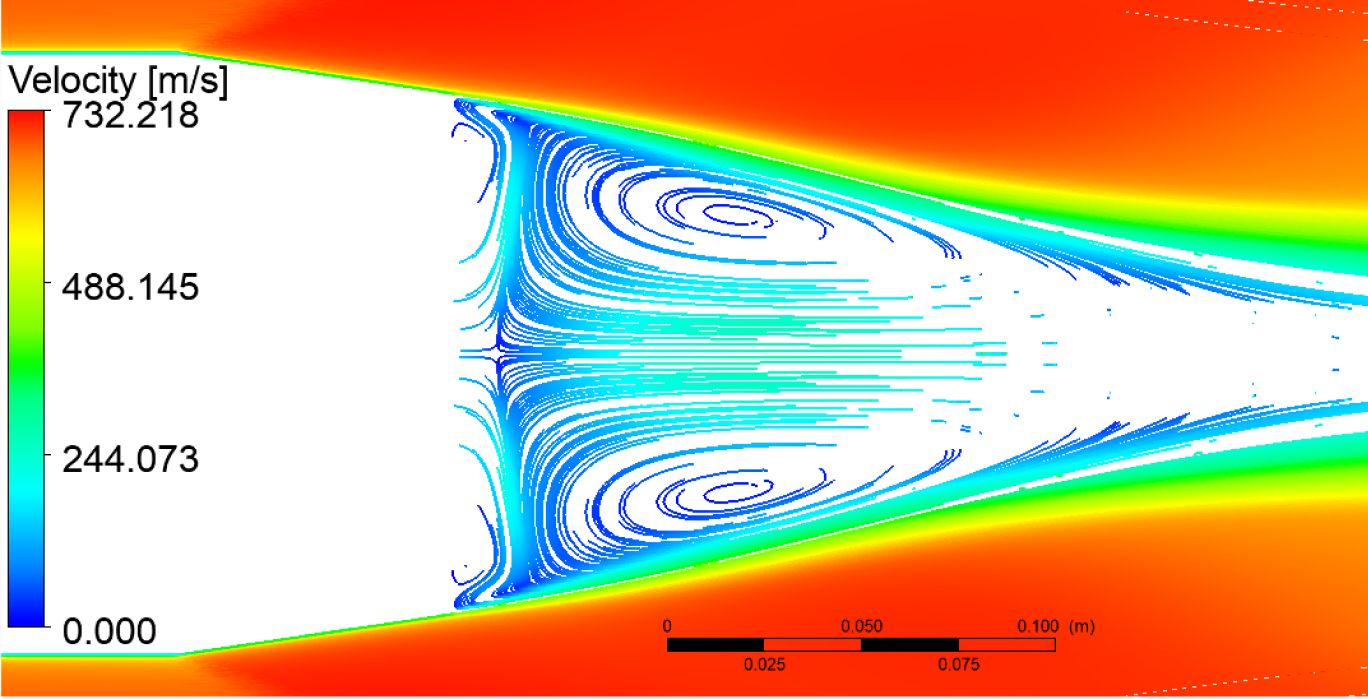
\includegraphics[height=5cm,width=\textwidth]{corrente-velocidade-2306K-vazao-0030-2pol.png}
        \caption{Linhas de corrente - \(\Dot{m}_{BB}\) = \qty{0,030}{\kilogram\per\second}}
        \label{fig:corrente-velocidade-bb-1500K-vazao0030}
    \end{subfigure}
    \hfill
    \begin{subfigure}[b]{0.47\textwidth} % FOTO 8
        \centering
        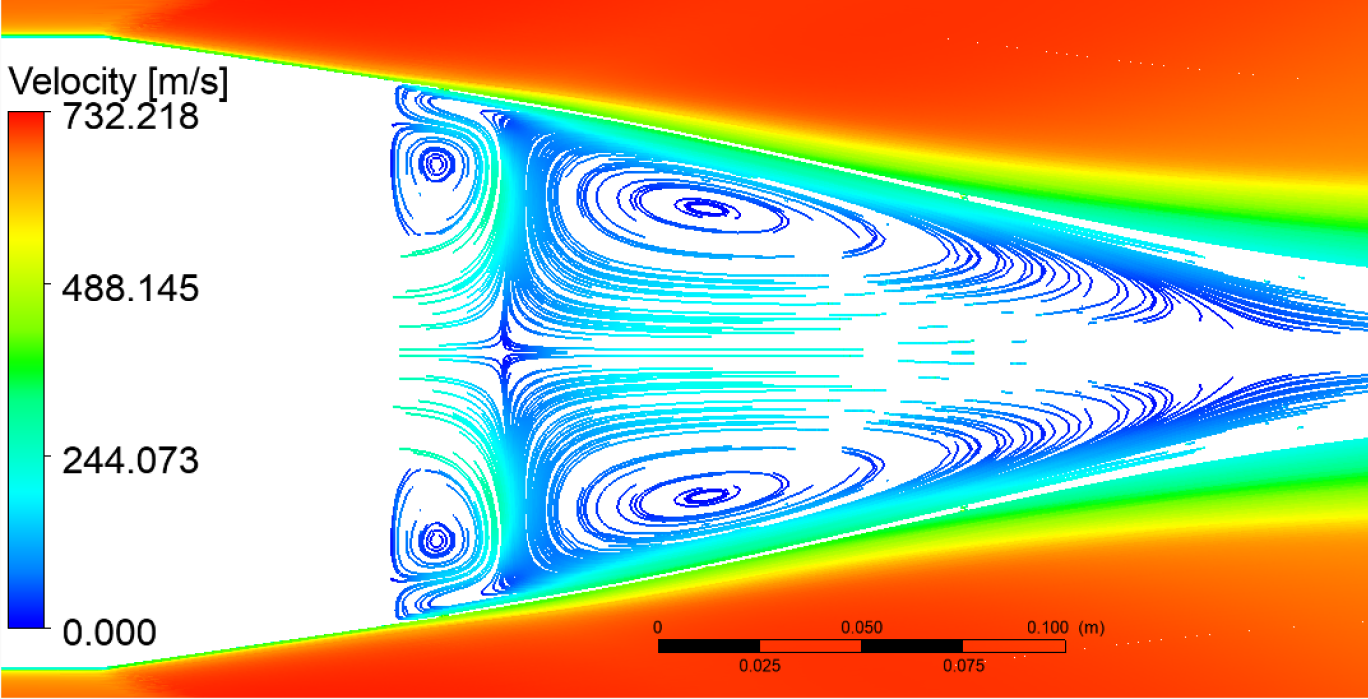
\includegraphics[height=5cm,width=\textwidth]{corrente-velocidade-2306K-vazao-0060-2pol.png}
        \caption{Linhas de corrente - \(\Dot{m}_{BB}\) = \qty{0,060}{\kilogram\per\second}}
        \label{fig:corrente-velocidade-bb-1500K-vazao0060}
    \end{subfigure}
    \caption{Campos de pressão e velocidade \(\left(\phi_{BB} = \qty{50,8}{\millimetre}; T_{BB} = \qty{1500}{\kelvin}\right)\)}
	\label{fig:influencia-vazao-bb}
\end{figure}

Assume-se o regime M = \num{2,0} para os campos de pressão e velocidade da \autoref{fig:influencia-vazao-bb}. Conforme aumenta a vazão, há um acréscimo de pressão, como pode ser visto tanto na \autoref{fig:contorno-pressao-base-bb-1500K-vazao0030} e \autoref{fig:contorno-pressao-base-bb-1500K-vazao0060}. Os contornos de velocidade, presentes na \autoref{fig:contorno-velocidade-bb-1500K-vazao0030} e \autoref{fig:contorno-velocidade-bb-1500K-vazao0060}, apresentam o deslocamento da região primária de recirculação, além do aumento da esteira turbulenta. Pelas Figuras \ref{fig:corrente-velocidade-bb-1500K-vazao0030} e \ref{fig:corrente-velocidade-bb-1500K-vazao0060} se observam as linhas de corrente para a velocidade. Em ambos os casos há a formação da recirculação anular, mas essa zona secundária de recirculação é mais proeminente conforme o aumento da vazão. A \autoref{fig:corrente-velocidade-bb-1500K-vazao0060} apresenta com maior clareza um valor mais próximo do que se espera ocorrer na região, dentro do que a literatura demonstrou em trabalhos anteriores \cite{Sahu1985,Andersson1976}.

\subsection{Influência da temperatura} \label{subsec:resultados-com-basebleed-temperatura}

A \autoref{fig:comparacao-basebleed-temperatura} demonstra a influência da temperatura nos resultados obtidos nas simulações computacionais com o efeito \textit{Base Bleed} na base do projetil, assumindo que a vazão mássica de saída dos gases foi fixada em \qty{0,060}{\kilogram\per\second} e o diâmetro de saída do \textit{Base Bleed} escolhido foi de \qty{2}{\polegada} \(\left(\phi_{BB} = \qty{50,8}{\millimetre}\right)\). A escolha por esse diâmetro de saída se deve aos melhores resultados produzidos na \autoref{subsec:resultados-com-basebleed-diametros}. A escolha pela vazão de \qty{0,060}{\kilogram\per\second} se baseou nos resultados das \autoref{subsec:resultados-com-basebleed-vazao}, em que a redução do coeficiente de arrasto foi mais significativo quando comparado ao projetil inerte.

\begin{figure}[!ht]
	\centering
	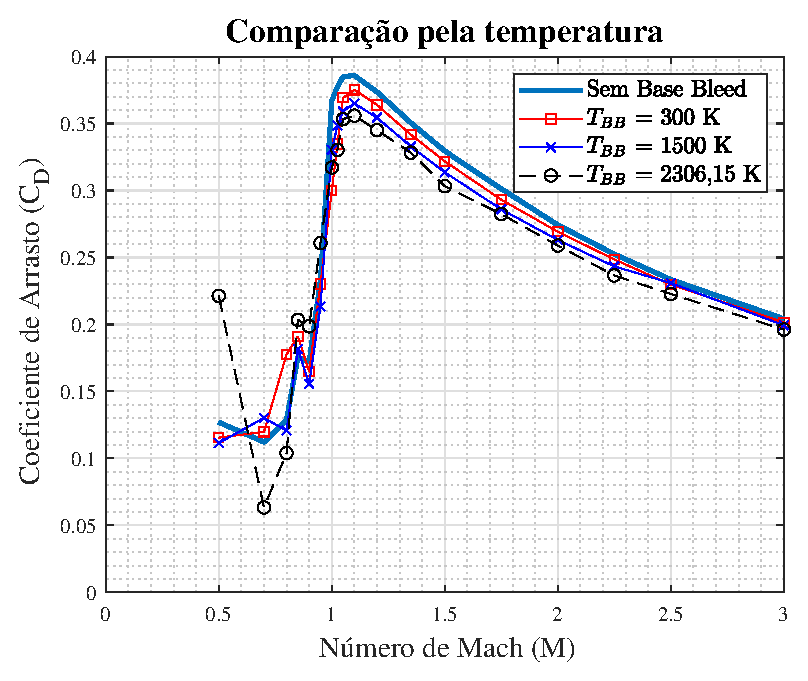
\includegraphics[width=0.5\textwidth]{cd-combasebleed-vazao006-2pol.eps}
	\caption{Influência da temperatura do \textit{Base Bleed} - \(\Dot{m}_{BB}\) = \qty{0,060}{\kilogram\per\second}}
	\label{fig:comparacao-basebleed-temperatura}
\end{figure}

A \autoref{fig:comparacao-basebleed-temperatura} mostra uma relação direta entre a redução de arrasto e a temperatura, \(T_{BB}\). O regime subsônico apresenta oscilações nas curvas de arrasto para os 3 casos com projetil ativo \(\left(T_{BB} = \qtylist{300;1500;2306,15}{\kelvin}\right)\) e essas variações são mais visíveis com o aumento da temperatura de saída dos gases, embora as flutuações sigam a mesma tendência. Assim como na Subseção~\ref{subsec:resultados-com-basebleed-vazao}, o regime transônico reuniu as maiores reduções de arrasto. A aplicação da tecnologia \textit{Base Bleed} produziu menor efeito com o aumento de velocidade no regime supersônico somente quando M \(\geq\) \num{2,5}.

\subsection{Influência da abordagem RANS}\label{subsec:resultados-com-basebleed-RANS}

O modelo Spalart-Allmaras \cite{Spalart1992} foi escolhido devido ao seu reconhecido uso em projetos aerodinâmicos, especialmente em estudos sobre velocidades supersônicas. O objetivo desta subseção é comparar a eficiência deste modelo RANS com o SST \(\kappa-\omega\) \cite{Menter1994TwoequationET,Menter2003,Menter2009}, já que é mais eficiente computacionalmente por ter apenas 1 equação de transporte para descrever a turbulência. Os parâmetros utilizados na comparação foram estabelecidos na condição de contorno \textit{Base Bleed inlet}: \(\phi_{BB}\) = \qty{50,8}{\millimetre}, \(T_{BB} = \qty{2306,15}{\kelvin}\) e \(\Dot{m}_{BB}\) = \qty{0,030}{\kilogram\per\second}.

\begin{figure}[!ht]
    \centering
    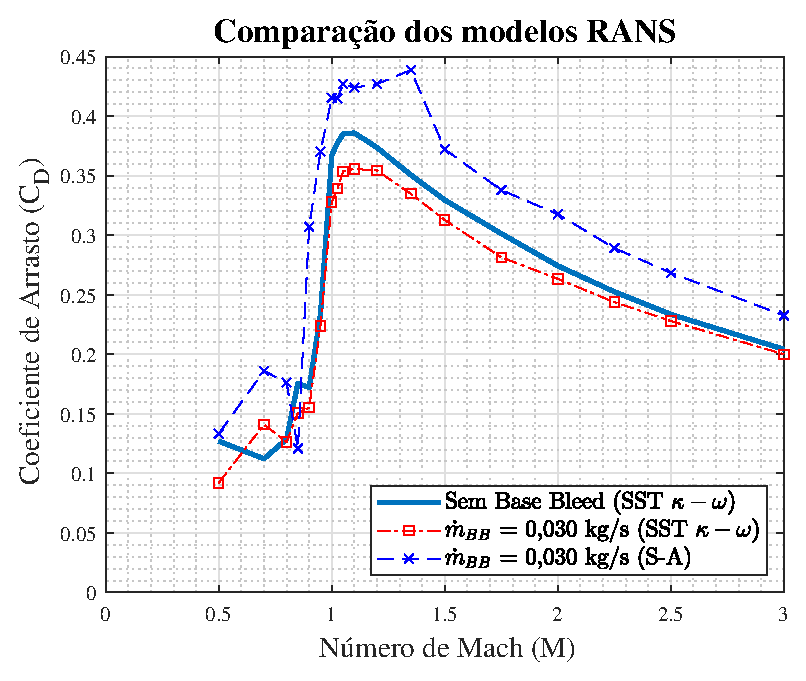
\includegraphics[width=0.5\textwidth]{cd-combasebleed-rans.eps}
 	\caption{Curvas de arrasto de acordo com modelos de turbulência RANS}
    \label{fig:comparacao-bb-rans}
\end{figure}

A \autoref{fig:comparacao-bb-rans} mostra como o modelo Spalart-Allmaras superestimou a curva de arrasto em todos os regimes de velocidade, inclusive quando se compara com o caso de referência (projetil inerte). Apesar de quantitativamente não ser aplicável para a predição de trajetória, os resultados para modelo S-A seguem a mesma tendência para o coeficiente de arrasto. Conclui-se que este modelo RANS é inadequado para analisar o perfil criado pelo jato do sistema \textit{Base Bleed}.

\begin{figure}[!htpb]
	\centering
	\begin{subfigure}[b]{0.47\textwidth}
        \centering
        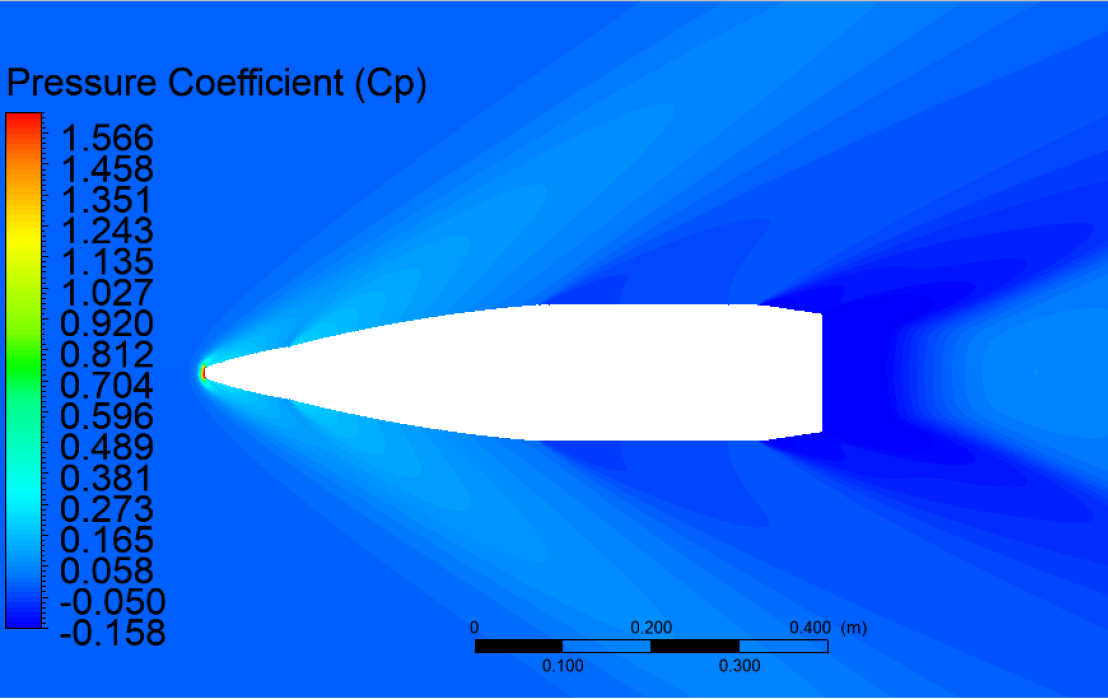
\includegraphics[height=5cm,width=\textwidth]{contorno-pressao-SPALART-2pol.png}
        \caption{Contornos de pressão}
        \label{fig:contorno-pressao-bb-2pol-RANS}
    \end{subfigure}
    \hfill
    \begin{subfigure}[b]{0.47\textwidth}
        \centering
        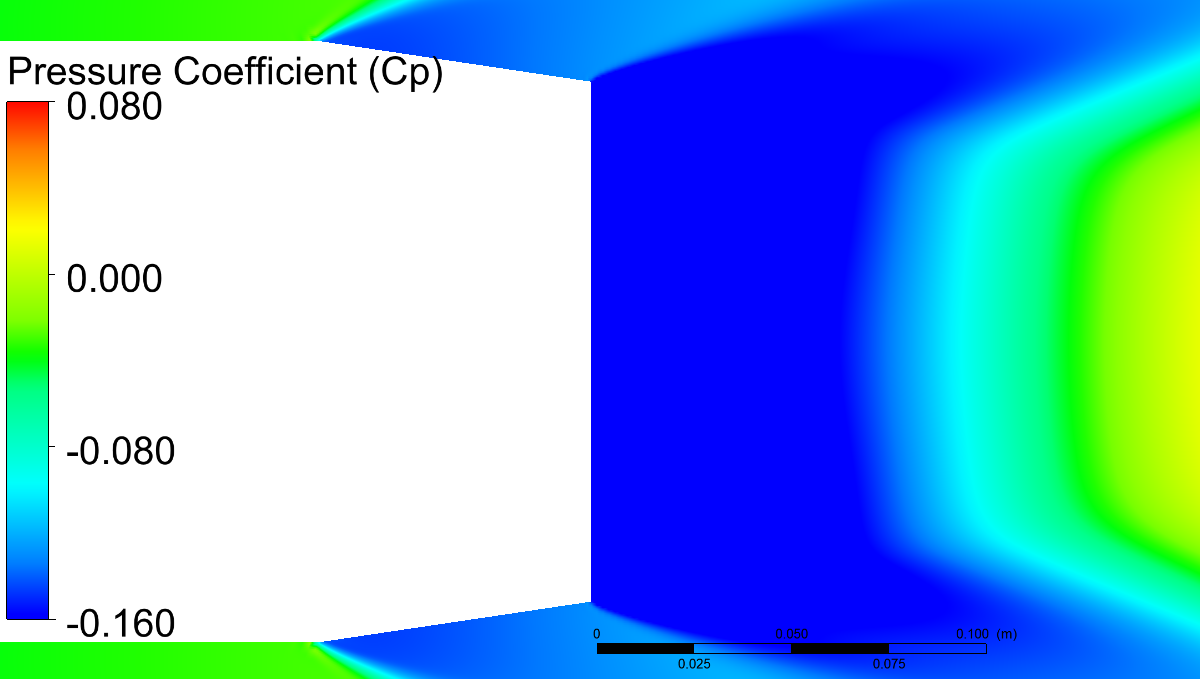
\includegraphics[height=5cm,width=\textwidth]{coeficientepressao-SPALART}
        \caption{Contornos de pressão}
        \label{fig:contorno-pressao-base-bb-2pol-RANS}
    \end{subfigure}
    \hfill
    \begin{subfigure}[b]{0.47\textwidth}
        \centering
        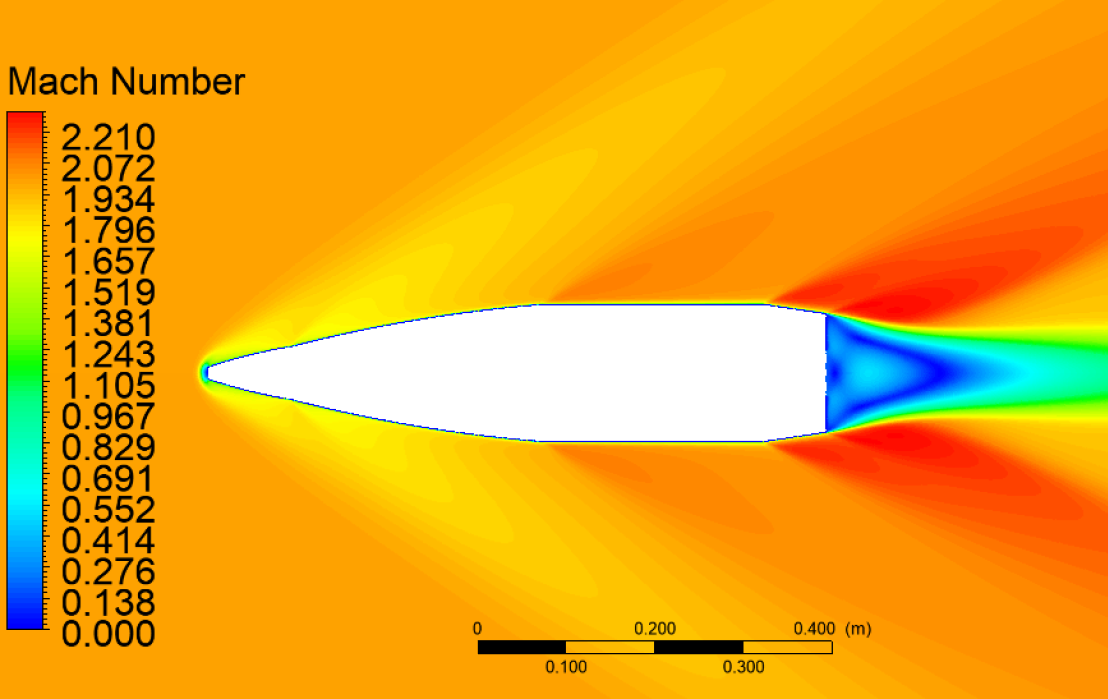
\includegraphics[height=5cm,width=\textwidth]{contorno-velocidade-SPALART-2pol.png}
        \caption{Contornos de velocidade}
        \label{fig:contorno-velocidade-bb-2pol-RANS}
    \end{subfigure}
    \hfill
    \begin{subfigure}[b]{0.47\textwidth}
        \centering
        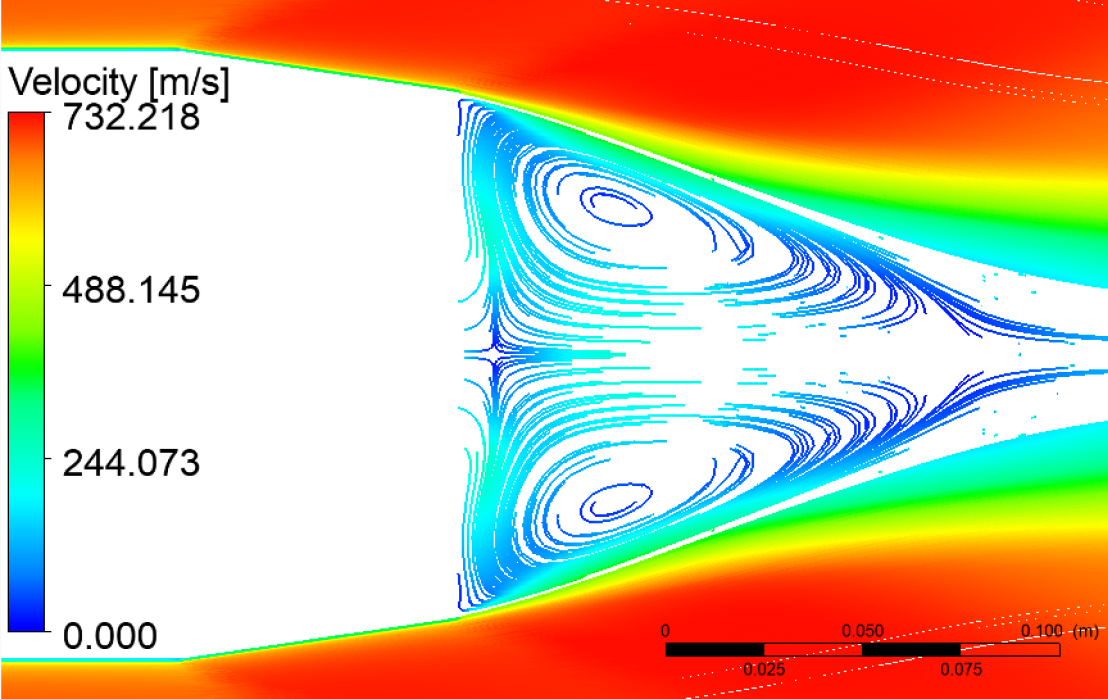
\includegraphics[height=5cm,width=\textwidth]{corrente-velocidade-SPALART-2pol.png}
        \caption{Linhas de corrente}
        \label{fig:corrente-velocidade-bb-2pol-RANS}
    \end{subfigure} 	
 	\caption{Linhas de corrente para o modelo Spalart-Allmaras}
    \label{fig:influencia-RANS-bb}
\end{figure}

A \autoref{fig:influencia-RANS-bb} apresenta o comportamento do \textit{Base Bleed} para M = \num{2,0} usando o modelo de 1 equação. O campo de pressão apresentado na \autoref{fig:contorno-pressao-bb-2pol-RANS} e com mais detalhes na \autoref{fig:contorno-pressao-base-bb-2pol-RANS} é subestimado, quando se avalia o resultado com o encontrado para o modelo SST \(\kappa-\omega\). Acerca do campo de velocidade, o modelo S-A não conseguiu captar a formação da região anular secundária de recirculação e tampouco o deslocamento da recirculação primária, como visto na \autoref{fig:contorno-velocidade-bb-2pol-RANS} e \autoref{fig:corrente-velocidade-bb-2pol-RANS}. O alto gradiente adverso de pressão existente na região a jusante da munição mostra a deficiência do modelo Spalart-Allmaras em analisar jatos turbulentos e bolhas de separação \cite{Wilcox2006}. 

\section{Resultados da Trajetória}\label{sec:resultados-trajetoria}

Os resultados encontrados nas simulações CFD do efeito \textit{Base Bleed} sobre a força de arrasto permitiram a implementação do modelo de trajetória com 4 graus de liberdade, o MPMTM. As curvas de arrasto escolhidas foram extraídas da \autoref{subsec:resultados-com-basebleed-diametros} por apresentarem diferenças que evidenciam a influência da vazão e do diâmetro de saída. Soma-se a esse fato os dados disponíveis na \autoref{subsec:implementacao-trajetoria} e do suporte do PRODAS® (ver Apêndices \ref{apend:apendice-sembb} a \ref{apend:apendice-combb-2pol-006}) para obter todas as informações necessárias, embora algumas premissas foram consideradas a partir de trabalhos anteriores \cite{Rosendo2020,ThallyoENCIT2022,DAVENAS1993329,RosendoCILAMCE2022}:

\begin{itemize}
    \item Lançamento do Rio de Janeiro, logo a latitude é de \ang{23};
    \item Os efeitos da umidade sobre a atmosfera são desprezíveis;
    \item Sem velocidade do vento;
    \item Vazão mássica do \textit{Base Bleed} é constante durante o acionamento;
    \item Parâmetro ótimo de injeção \(\left(Inj_{0}\right)\) igual a \num{5e-3};
    \item Os coeficientes aerodinâmicos são linearmente dependentes do ângulo \(\alpha_{e}\).
\end{itemize}

Pela última condição assumida, logo \(C_{L\alpha^{3}}\) e \(C_{m\alpha^{3}}\) não interferem significativamente as equações \ref{eq:liftMPM} e \ref{eq:guinada-de-reposicao}. Embora a ignição seja um tópico relevante no desempenho, a dificuldade em modelar adequadamente à realidade tornou o assunto um caso a ser tratado em estudos posteriores. O mesmo também vale para os fatores \(f_{L}\) e \(i_{BB}\), que servem de ajustes às equações \ref{eq:liftMPM} e \ref{eq:baseMPM}.

A \autoref{tab:tabela-validacao-PRODAS-e-tabela-de-tiro-M107} serve para validar o código desenvolvido em MATLAB®. Os resultados de alcance foram comparados com o PRODAS® e uma tabela de tiro de acordo com ângulos de elevação. Os erros superiores a \qty{1}{\percent} foram vistos em grandes elevações (QE \(\approx\) \qty{1200}{\milliradian}), donde se espera inconsistências~\cite{McCoy2012,Carlucci2018}.

\begin{table}[ht]
    \centering
    \caption[Resultados obtidos durante a validação (munição \qty{155}{\millimetre} M107)]{Resultados obtidos durante a validação (munição \qty{155}{\millimetre} M107)}
    \vspace{0.5cm}
    \resizebox{\textwidth}{!}{%
    \begin{tabular}{c|c|c|c|c|c|c|c}
        \hline
        \multicolumn{4}{c|}{PRODAS®} &
        \multicolumn{4}{c}{Tabela de tiro} \\ 
        \hline
        \multicolumn{1}{c|}{\multirow{2}{*}{\begin{tabular}[c]{@{}c@{}}Elevação \\ (\unit{\milliradian})\end{tabular}}} & \multicolumn{2}{c|}{Alcance (\unit{\metre})} & \multirow{2}{*}{\begin{tabular}[c]{@{}c@{}}Erro \\ (\unit{\percent})\end{tabular}} & \multicolumn{1}{c|}{\multirow{2}{*}{\begin{tabular}[c]{@{}c@{}}Elevação \\ (\unit{\milliradian})\end{tabular}}} & \multicolumn{2}{c|}{Alcance (\unit{\metre})} & \multirow{2}{*}{\begin{tabular}[c]{@{}c@{}}Erro \\ (\unit{\percent})\end{tabular}} \\
        \cline{2-3} \cline{6-7}
        \multicolumn{1}{c|}{} & \multicolumn{1}{c|}{Esperado} & \multicolumn{1}{c|}{Obtido} & & \multicolumn{1}{c|}{} & \multicolumn{1}{c|}{Esperado} & \multicolumn{1}{c|}{Obtido} & \\ 
        \hline
        \num{58,9} & \num{500,0} & \num{501,2} & \num{0,24} & \num{58,9} & \num{500,0} & \num{501,2} & \num{0,24} \\
        \num{120,1} & \num{1000,0} & \num{1001,9} & \num{0,19} & \num{120,3} & \num{1000,0} & \num{1003,5} & \num{0,35} \\
        \num{184,7} & \num{1500,0} & \num{1501,7} & \num{0,11} & \num{185,3} & \num{1500,0} & \num{1506,2} & \num{0,41} \\
        \num{254,5} & \num{2000,0} & \num{2001,7} & \num{0,09} & \num{255,4} & \num{2000,0} & \num{2007,9} & \num{0,40} \\
        \num{332,1} & \num{2500,0} & \num{2501,1} & \num{0,04} & \num{333,5} & \num{2500,0} & \num{2509,5} & \num{0,38} \\
        \num{422,9} & \num{3000,0} & \num{2999,9} & \num{0,00} & \num{424,7} & \num{3000,0} & \num{3008,8} & \num{0,29} \\
        \num{541,9} & \num{3500,0} & \num{3498,9} & \num{0,03} & \num{543,8} & \num{3500,0} & \num{3505,3} & \num{0,15} \\
        \num{731,3} & \num{3900,0} & \num{3897,6} & \num{0,06} & \num{729,2} & \num{3900,0} & \num{3896,0} & \num{0,11} \\
        \num{838,4} & \num{3900,0} & \num{3898,3} & \num{0,05} & \num{846,2} & \num{3900,0} & \num{3891,9} & \num{0,21} \\
        \num{1027,5} & \num{3500,0} & \num{3504,3} & \num{0,11} & \num{1028,3} & \num{3500,0} & \num{3501,5} & \num{0,03} \\
        \num{1144,7} & \num{3000,0} & \num{3016,7} & \num{0,53} & \num{1141,1} & \num{3000,0} & \num{3034,3} & \num{1,12} \\
        \num{1231,4} & \num{2500,0} & \num{2539,9} & \num{1,55} & \num{1220,5} & \num{2500,0} & \num{2605,5} & \num{4,18} \\ 
        \hline
    \end{tabular}%
    }
    \label{tab:tabela-validacao-PRODAS-e-tabelaS-de-tiro-M107}
    \fonte{Autor.}
\end{table}

A metodologia para provar a eficiência do \textit{Base Bleed} foi demonstrar os alcances obtidos em simulações computacionais. A \autoref{fig:trajetoria-711mil-comparacao} esclarece os resultados das predições de voo para uma munição a QE = \qty{711}{\milliradian} e v = \qty{878}{\metre\per\second} (M = \num{2,58} a nível do mar). Os valores máximos de alcance horizontal e apogeu são expostos na  \autoref{tab:tabela-711mil-bb-1e2pol}.

\begin{figure}[!htpb]
	\centering
    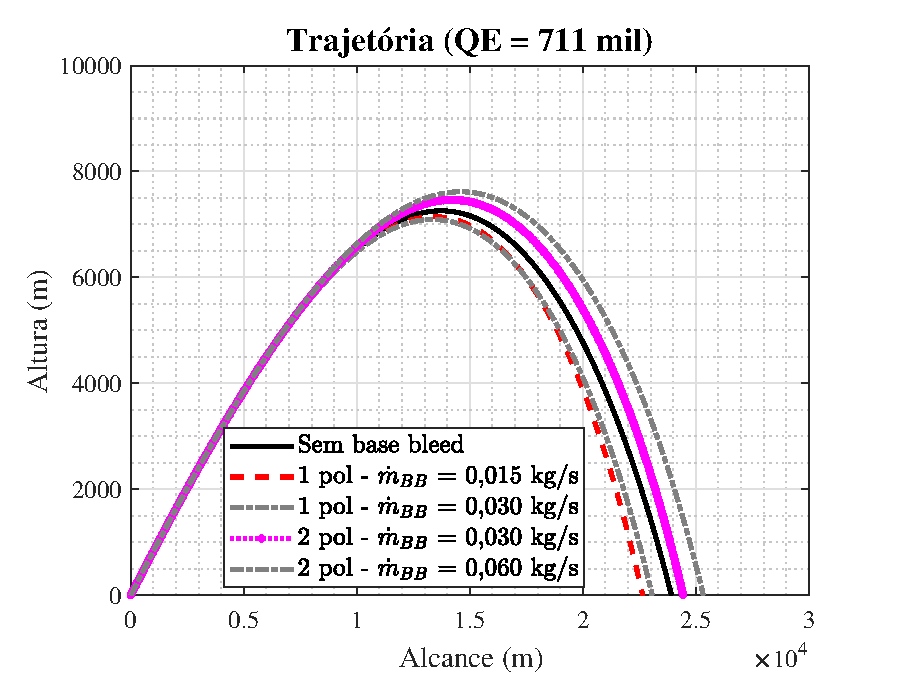
\includegraphics[width=0.75\textwidth]{foto1-qe711mil-comparacao.eps}
    \caption[QE = \qty{711}{\milliradian}]{QE = \qty{711}{\milliradian}}
    \label{fig:trajetoria-711mil-comparacao}
\end{figure}

\begin{table}[!htpb]
    \centering
    \caption[Trajetória Balística com QE = \qty{711}{\milliradian} e v = \qty{878}{\metre\per\second}]{Trajetória Balística com QE = \qty{711}{\milliradian} e v = \qty{878}{\metre\per\second}}
    \vspace{0.5cm}
    \begin{tabular}{c|c|c|c|c|c}
        \hline
        Diâmetro \textit{Base Bleed} & Vazão Mássica & Alcance & Aumento & Apogeu & Aumento \\
        \hline
        Inerte & \qty{0}{\kilogram\per\second} & \qty{23922,2}{\metre} & -- & \qty{7256,8}{\metre} & -- \\ 
        \multirow{2}{*}{\qty{25,4}{\millimetre}} & \qty{0,015}{\kilogram\per\second} & \qty{22647,8}{\metre} & \qty{-5,3}{\percent} & \qty{7145,0}{\metre} & \qty{-1,5}{\percent} \\
        & \qty{0,030}{\kilogram\per\second} & \qty{23069,0}{\metre} & \qty{-3,6}{\percent} & \qty{7093,4}{\metre} & \qty{-2,3}{\percent} \\
        \multirow{2}{*}{\qty{50,8}{\millimetre}} & \qty{0,030}{\kilogram\per\second} & \qty{24439,8}{\metre} & \qty{2,2}{\percent} & \qty{7463,5}{\metre} & \qty{2,8}{\percent} \\
        & \qty{0,060}{\kilogram\per\second} & \qty{25334,3}{\metre} & \qty{5,9}{\percent} & \qty{7616,6}{\metre} & \qty{5,0}{\percent} \\
        \hline
    \end{tabular}
    \label{tab:tabela-711mil-bb-1e2pol}
    \fonte{Autor.}   
\end{table}

Ao observar as predições de trajetória expostos na \autoref{fig:trajetoria-711mil-comparacao} percebe-se que o \textit{Base Bleed} com \(\phi_{BB} = \qty{25,4}{\millimetre}\) provoca uma redução de desempenho, se comparado aos resultados do projetil inerte. Por outro lado, o aumento do diâmetro de \num{25,4} para \qty{50,8}{\millimetre} resulta no aumento de desempenho, seja no deslocamento horizontal ou vertical. Além disso, verifica-se que há uma relação direta entre a vazão mássica e a extensão de alcance da munição.

Acerca da \autoref{fig:trajetoria-800mil-comparacao}, também há uma redução de desempenho ao implementar o \textit{Base Bleed} com \(\phi_{BB} = \qty{25,4}{\millimetre}\).  A \autoref{tab:tabela-800mil-bb-1e2pol} descreve os resultados. Para o alcance a maior diferença ficou em aproximadamente \qty{1312}{\metre}, enquanto que para o apogeu o menor valor foi de \qty{202,7}{\metre}.

\begin{figure}[!htpb]
	\centering
    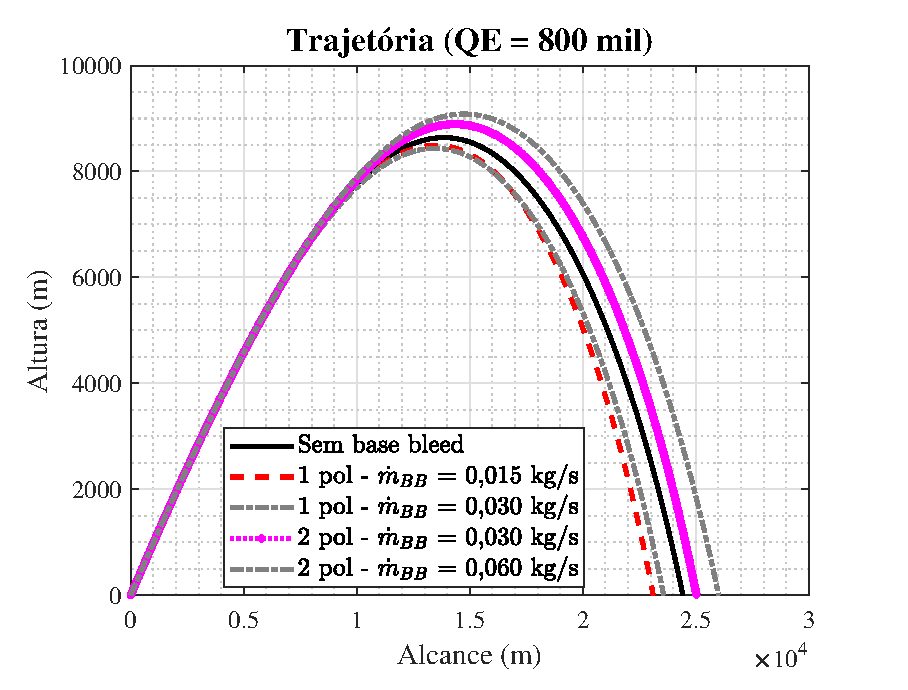
\includegraphics[width=0.75\textwidth]{foto2-qe800mil-comparacao.eps}
    \caption[QE = \qty{800}{\milliradian} \(\left(\phi_{BB} = \qty{25,4}{\millimetre}\right)\)]{QE = \qty{800}{\milliradian}}
    \label{fig:trajetoria-800mil-comparacao}
\end{figure}

Ao verificar os resultados do projetil com \(\phi_{BB} = \qty{50,8}{\millimetre}\), percebe-se um aumento do alcance e do apogeu, atestado nas Tabelas \ref{tab:tabela-711mil-bb-1e2pol} e \ref{tab:tabela-800mil-bb-1e2pol}. Há o aumento do alcance de quase \qty{6}{\percent} quando \(\Dot{m}_{BB} = \qty{0,060}{\kilogram\per\second}\). Ao aumentar o ângulo de elevação para \qty{800}{\milliradian} houve um incremento percentual sobre o alcance e o apogeu também, como demonstrado na \autoref{fig:trajetoria-800mil-comparacao}. Os resultados seguiram a mesma ordem de crescimento do deslocamento, quando se compara a \autoref{tab:tabela-711mil-bb-1e2pol} com a \autoref{tab:tabela-800mil-bb-1e2pol}. De qualquer forma, o diâmetro de saída do bocal tem forte influência na balística externa do projetil.

\begin{table}[!htpb]
    \centering
    \caption[Trajetória Balística com QE = \qty{800}{\milliradian} e v = \qty{878}{\metre\per\second}]{Trajetória Balística com QE = \qty{800}{\milliradian} e v = \qty{878}{\metre\per\second}}
    \vspace{0.5cm}
    \begin{tabular}{c|c|c|c|c|c}
        \hline
        Diâmetro \textit{Base Bleed} & Vazão Mássica & Alcance & Aumento & Apogeu & Aumento \\
        \hline
        Inerte & \qty{0}{\kilogram\per\second} & \qty{24429,5}{\metre} & -- & \qty{8638,6}{\metre} & -- \\ 
        \multirow{2}{*}{\qty{25,4}{\millimetre}} & \qty{0,015}{\kilogram\per\second} & \qty{23117,9}{\metre} & \qty{-5,4}{\percent} & \qty{8493,6}{\metre} & \qty{-1,7}{\percent} \\
        & \qty{0,030}{\kilogram\per\second} & \qty{23577,0}{\metre} & \qty{-3,5}{\percent} & \qty{8435,9}{\metre} & \qty{-2,3}{\percent} \\
        \multirow{2}{*}{\qty{50,8}{\millimetre}} & \qty{0,030}{\kilogram\per\second} & \qty{25030,7}{\metre} & \qty{2,5}{\percent} & \qty{8892,7}{\metre} & \qty{2,9}{\percent} \\
        & \qty{0,060}{\kilogram\per\second} & \qty{26008,5}{\metre} & \qty{6,5}{\percent} & \qty{9084,5}{\metre} & \qty{5,2}{\percent} \\
        \hline
    \end{tabular}
    \label{tab:tabela-800mil-bb-1e2pol}
    \fonte{Autor.}
\end{table}

